\documentclass{article}

%%%%%%%%%%%%%%%%%%%%%%%%%%%%%%%%%
% PACKAGE IMPORTS
%%%%%%%%%%%%%%%%%%%%%%%%%%%%%%%%%
\usepackage[tmargin=2cm,rmargin=1in,lmargin=1in,margin=0.85in,bmargin=2cm,footskip=.2in]{geometry}
\usepackage{amsmath,amsfonts,amsthm,amssymb,mathtools}
\usepackage[varbb]{newpxmath}
\usepackage{xfrac}
\usepackage[makeroom]{cancel}
\usepackage{mathtools}
\usepackage{bookmark}
\usepackage{enumitem}
\usepackage{hyperref,theoremref}
\hypersetup{
	pdftitle={Assignment},
	colorlinks=true, linkcolor=doc!90,
	bookmarksnumbered=true,
	bookmarksopen=true
}
\graphicspath{ {./images/} }
\usepackage[most,many,breakable]{tcolorbox}
\usepackage{xcolor}
\usepackage{varwidth}
\usepackage{varwidth}
\usepackage{etoolbox}
\usepackage{nameref}
\usepackage{multicol,array}
\usepackage{tikz-cd}
\usepackage[ruled,vlined,linesnumbered]{algorithm2e}
\usepackage{comment} % enables the use of multi-line comments (\ifx \fi) 
\usepackage{import}
\usepackage{xifthen}
\usepackage{pdfpages}
\usepackage{transparent}
\usepackage{tikzsymbols}
\usepackage{fix-cm}

%%%%%%%%%%%%%%%%%%%%%%%%%%%%%%
% SELF MADE COLORS
%%%%%%%%%%%%%%%%%%%%%%%%%%%%%%

\definecolor{myg}{RGB}{56, 140, 70}
\definecolor{myb}{RGB}{45, 111, 177}
\definecolor{myr}{RGB}{199, 68, 64}
\definecolor{mytheorembg}{HTML}{F2F2F9}
\definecolor{mytheoremfr}{HTML}{00007B}
\definecolor{mylenmabg}{HTML}{FFFAF8}
\definecolor{mylenmafr}{HTML}{983b0f}
\definecolor{mypropbg}{HTML}{f2fbfc}
\definecolor{mypropfr}{HTML}{191971}
\definecolor{myexamplebg}{HTML}{F2FBF8}
\definecolor{myexamplefr}{HTML}{88D6D1}
\definecolor{myexampleti}{HTML}{2A7F7F}
\definecolor{mydefinitbg}{HTML}{E5E5FF}
\definecolor{mydefinitfr}{HTML}{3F3FA3}
\definecolor{notesgreen}{RGB}{0,162,0}
\definecolor{myp}{RGB}{197, 92, 212}
\definecolor{mygr}{HTML}{2C3338}
\definecolor{myred}{RGB}{127,0,0}
\definecolor{myyellow}{RGB}{169,121,69}
\definecolor{myexercisebg}{HTML}{F2FBF8}
\definecolor{myexercisefg}{HTML}{88D6D1}


\setlength{\parindent}{1cm}
%================================
% EXAMPLE BOX
%================================

\newtcbtheorem[number within=section]{Example}{Example}
{%
	colback = myexamplebg
	,breakable
	,colframe = myexamplefr
	,coltitle = myexampleti
	,boxrule = 1pt
	,sharp corners
	,detach title
	,before upper=\tcbtitle\par\smallskip
	,fonttitle = \bfseries
	,description font = \mdseries
	,separator sign none
	,description delimiters parenthesis
}
{ex}

%================================
% DEFINITION BOX
%================================

\newtcbtheorem[number within=section]{Definition}{Definition}{enhanced,
	before skip=2mm,after skip=2mm, colback=red!5,colframe=red!80!black,boxrule=0.5mm,
	attach boxed title to top left={xshift=1cm,yshift*=1mm-\tcboxedtitleheight}, varwidth boxed title*=-3cm,
	boxed title style={frame code={
					\path[fill=tcbcolback]
					([yshift=-1mm,xshift=-1mm]frame.north west)
					arc[start angle=0,end angle=180,radius=1mm]
					([yshift=-1mm,xshift=1mm]frame.north east)
					arc[start angle=180,end angle=0,radius=1mm];
					\path[left color=tcbcolback!60!black,right color=tcbcolback!60!black,
						middle color=tcbcolback!80!black]
					([xshift=-2mm]frame.north west) -- ([xshift=2mm]frame.north east)
					[rounded corners=1mm]-- ([xshift=1mm,yshift=-1mm]frame.north east)
					-- (frame.south east) -- (frame.south west)
					-- ([xshift=-1mm,yshift=-1mm]frame.north west)
					[sharp corners]-- cycle;
				},interior engine=empty,
		},
	fonttitle=\bfseries,
	title={#2},#1}{def}

%================================
% Solution BOX
%================================

\makeatletter
\newtcbtheorem[number within=section]{question}{Question}{enhanced,
	breakable,
	colback=white,
	colframe=myb!80!black,
	attach boxed title to top left={yshift*=-\tcboxedtitleheight},
	fonttitle=\bfseries,
	title={#2},
	boxed title size=title,
	boxed title style={%
			sharp corners,
			rounded corners=northwest,
			colback=tcbcolframe,
			boxrule=0pt,
		},
	underlay boxed title={%
			\path[fill=tcbcolframe] (title.south west)--(title.south east)
			to[out=0, in=180] ([xshift=5mm]title.east)--
			(title.center-|frame.east)
			[rounded corners=\kvtcb@arc] |-
			(frame.north) -| cycle;
		},
	#1
}{def}
\makeatother

%================================
% SOLUTION BOX
%================================

\makeatletter
\newtcolorbox{solution}{enhanced,
	breakable,
	colback=white,
	colframe=myg!80!black,
	attach boxed title to top left={yshift*=-\tcboxedtitleheight},
	title=Solution,
	boxed title size=title,
	boxed title style={%
			sharp corners,
			rounded corners=northwest,
			colback=tcbcolframe,
			boxrule=0pt,
		},
	underlay boxed title={%
			\path[fill=tcbcolframe] (title.south west)--(title.south east)
			to[out=0, in=180] ([xshift=5mm]title.east)--
			(title.center-|frame.east)
			[rounded corners=\kvtcb@arc] |-
			(frame.north) -| cycle;
		},
}
\makeatother

%================================
% Question BOX
%================================

\makeatletter
\newtcbtheorem{qstion}{Question}{enhanced,
	breakable,
	colback=white,
	colframe=mygr,
	attach boxed title to top left={yshift*=-\tcboxedtitleheight},
	fonttitle=\bfseries,
	title={#2},
	boxed title size=title,
	boxed title style={%
			sharp corners,
			rounded corners=northwest,
			colback=tcbcolframe,
			boxrule=0pt,
		},
	underlay boxed title={%
			\path[fill=tcbcolframe] (title.south west)--(title.south east)
			to[out=0, in=180] ([xshift=5mm]title.east)--
			(title.center-|frame.east)
			[rounded corners=\kvtcb@arc] |-
			(frame.north) -| cycle;
		},
	#1
}{def}
\makeatother

\newtcbtheorem[number within=chapter]{wconc}{Wrong Concept}{
	breakable,
	enhanced,
	colback=white,
	colframe=myr,
	arc=0pt,
	outer arc=0pt,
	fonttitle=\bfseries\sffamily\large,
	colbacktitle=myr,
	attach boxed title to top left={},
	boxed title style={
			enhanced,
			skin=enhancedfirst jigsaw,
			arc=3pt,
			bottom=0pt,
			interior style={fill=myr}
		},
	#1
}{def}

%================================
% NOTE BOX
%================================

\usetikzlibrary{arrows,calc,shadows.blur}
\tcbuselibrary{skins}
\newtcolorbox{note}[1][]{%
	enhanced jigsaw,
	colback=gray!20!white,%
	colframe=gray!80!black,
	size=small,
	boxrule=1pt,
	title=\textbf{Note:-},
	halign title=flush center,
	coltitle=black,
	breakable,
	drop shadow=black!50!white,
	attach boxed title to top left={xshift=1cm,yshift=-\tcboxedtitleheight/2,yshifttext=-\tcboxedtitleheight/2},
	minipage boxed title=1.5cm,
	boxed title style={%
			colback=white,
			size=fbox,
			boxrule=1pt,
			boxsep=2pt,
			underlay={%
					\coordinate (dotA) at ($(interior.west) + (-0.5pt,0)$);
					\coordinate (dotB) at ($(interior.east) + (0.5pt,0)$);
					\begin{scope}
						\clip (interior.north west) rectangle ([xshift=3ex]interior.east);
						\filldraw [white, blur shadow={shadow opacity=60, shadow yshift=-.75ex}, rounded corners=2pt] (interior.north west) rectangle (interior.south east);
					\end{scope}
					\begin{scope}[gray!80!black]
						\fill (dotA) circle (2pt);
						\fill (dotB) circle (2pt);
					\end{scope}
				},
		},
	#1,
}

%================================
% THEOREM BOX
%================================

\tcbuselibrary{theorems,skins,hooks}
\newtcbtheorem[number within=section]{Theorem}{Theorem}
{%
	enhanced,
	breakable,
	colback = mytheorembg,
	frame hidden,
	boxrule = 0sp,
	borderline west = {2pt}{0pt}{mytheoremfr},
	sharp corners,
	detach title,
	before upper = \tcbtitle\par\smallskip,
	coltitle = mytheoremfr,
	fonttitle = \bfseries\sffamily,
	description font = \mdseries,
	separator sign none,
	segmentation style={solid, mytheoremfr},
}
{th}

%================================
% Custom
%================================

\newcommand{\ex}[2]{\begin{Example}{#1}{}#2\end{Example}}
\newcommand{\dfn}[2]{\begin{Definition}[colbacktitle=red!75!black]{#1}{}#2\end{Definition}}
\newcommand{\qs}[2]{\begin{question}{#1}{}#2\end{question}}
\newcommand{\nt}[1]{\begin{note}#1\end{note}}
\newcommand{\thm}[2]{\begin{Theorem}{#1}{}#2\end{Theorem}}
\newcommand{\pf}[2]{\begin{myproof}[#1]#2\end{myproof}}

\newenvironment{myproof}[1][\proofname]{%
	\proof[\bfseries #1: ]%
}{\endproof}

\newcommand{\imgg}[2]{\begin{center}\includegraphics[scale=#2]{#1}\end{center}}
\newcommand{\al}[1]{\begin{align*} #1 \end{align*}}
%From M275 "Topology" at SJSU
\newcommand{\id}{\mathrm{id}}
\newcommand{\taking}[1]{\xrightarrow{#1}}
\newcommand{\inv}{^{-1}}

%From M170 "Introduction to Graph Theory" at SJSU
\DeclareMathOperator{\diam}{diam}
\DeclareMathOperator{\ord}{ord}
\newcommand{\defeq}{\overset{\mathrm{def}}{=}}

%From the USAMO .tex files
\newcommand{\ts}{\textsuperscript}
\newcommand{\dg}{^\circ}
\newcommand{\ii}{\item}

% % From Math 55 and Math 145 at Harvard
% \newenvironment{subproof}[1][Proof]{%
% \begin{proof}[#1] \renewcommand{\qedsymbol}{$\blacksquare$}}%
% {\end{proof}}

\newcommand{\ihat}{\hat{i}}
\newcommand{\jhat}{\hat{j}}
\newcommand{\khat}{\hat{k}}

\newcommand{\liff}{\leftrightarrow}
\newcommand{\lthen}{\rightarrow}
\newcommand{\opname}{\operatorname}
\newcommand{\surjto}{\twoheadrightarrow}
\newcommand{\injto}{\hookrightarrow}
\newcommand{\On}{\mathrm{On}} % ordinals
\DeclareMathOperator{\img}{im} % Image
\DeclareMathOperator{\Img}{Im} % Image
\DeclareMathOperator{\coker}{coker} % Cokernel
\DeclareMathOperator{\Coker}{Coker} % Cokernel
\DeclareMathOperator{\Ker}{Ker} % Kernel
\DeclareMathOperator{\rank}{rank}
\DeclareMathOperator{\Spec}{Spec} % spectrum
\DeclareMathOperator{\Tr}{Tr} % trace
\DeclareMathOperator{\pr}{pr} % projection
\DeclareMathOperator{\ext}{ext} % extension
\DeclareMathOperator{\pred}{pred} % predecessor
\DeclareMathOperator{\dom}{dom} % domain
\DeclareMathOperator{\ran}{ran} % range
\DeclareMathOperator{\Hom}{Hom} % homomorphism
\DeclareMathOperator{\Mor}{Mor} % morphisms
\DeclareMathOperator{\End}{End} % endomorphism

\newcommand{\eps}{\epsilon}
\newcommand{\veps}{\varepsilon}
\newcommand{\ol}{\overline}
\newcommand{\ul}{\underline}
\newcommand{\wt}{\widetilde}
\newcommand{\wh}{\widehat}
\newcommand{\vocab}[1]{\textbf{\color{blue} #1}}
\providecommand{\half}{\frac{1}{2}}
\newcommand{\dang}{\measuredangle} %% Directed angle
\newcommand{\ray}[1]{\overrightarrow{#1}}
\newcommand{\seg}[1]{\overline{#1}}
\newcommand{\arc}[1]{\wideparen{#1}}
\DeclareMathOperator{\cis}{cis}
\DeclareMathOperator*{\lcm}{lcm}
\DeclareMathOperator*{\argmin}{arg min}
\DeclareMathOperator*{\argmax}{arg max}
\newcommand{\cycsum}{\sum_{\mathrm{cyc}}}
\newcommand{\symsum}{\sum_{\mathrm{sym}}}
\newcommand{\cycprod}{\prod_{\mathrm{cyc}}}
\newcommand{\symprod}{\prod_{\mathrm{sym}}}
\newcommand{\Qed}{\begin{flushright}\qed\end{flushright}}
\newcommand{\parinn}{\setlength{\parindent}{1cm}}
\newcommand{\parinf}{\setlength{\parindent}{0cm}}
% \newcommand{\norm}{\|\cdot\|}
\newcommand{\inorm}{\norm_{\infty}}
\newcommand{\opensets}{\{V_{\alpha}\}_{\alpha\in I}}
\newcommand{\oset}{V_{\alpha}}
\newcommand{\opset}[1]{V_{\alpha_{#1}}}
\newcommand{\lub}{\text{lub}}
\newcommand{\del}[2]{\frac{\partial #1}{\partial #2}}
\newcommand{\Del}[3]{\frac{\partial^{#1} #2}{\partial^{#1} #3}}
\newcommand{\deld}[2]{\dfrac{\partial #1}{\partial #2}}
\newcommand{\Deld}[3]{\dfrac{\partial^{#1} #2}{\partial^{#1} #3}}
\newcommand{\lm}{\lambda}
\newcommand{\uin}{\mathbin{\rotatebox[origin=c]{90}{$\in$}}}
\newcommand{\usubset}{\mathbin{\rotatebox[origin=c]{90}{$\subset$}}}
\newcommand{\lt}{\left}
\newcommand{\rt}{\right}
\newcommand{\bs}[1]{\boldsymbol{#1}}
\newcommand{\exs}{\exists}
\newcommand{\st}{\strut}
\newcommand{\dps}[1]{\displaystyle{#1}}

\newcommand{\sol}{\setlength{\parindent}{0cm}\textbf{\textit{Solution:}}\setlength{\parindent}{1cm} }
\newcommand{\solve}[1]{\setlength{\parindent}{0cm}\textbf{\textit{Solution: }}\setlength{\parindent}{1cm}#1 \Qed}

\newcommand{\double}{\\\\}
\newcommand{\triple}{\\\\\\}
% Things Lie
\newcommand{\kb}{\mathfrak b}
\newcommand{\kg}{\mathfrak g}
\newcommand{\kh}{\mathfrak h}
\newcommand{\kn}{\mathfrak n}
\newcommand{\ku}{\mathfrak u}
\newcommand{\kz}{\mathfrak z}
\DeclareMathOperator{\Ext}{Ext} % Ext functor
\DeclareMathOperator{\Tor}{Tor} % Tor functor
\newcommand{\gl}{\opname{\mathfrak{gl}}} % frak gl group
\renewcommand{\sl}{\opname{\mathfrak{sl}}} % frak sl group chktex 6

% More script letters etc.
\newcommand{\SA}{\mathcal A}
\newcommand{\SB}{\mathcal B}
\newcommand{\SC}{\mathcal C}
\newcommand{\SF}{\mathcal F}
\newcommand{\SG}{\mathcal G}
\newcommand{\SH}{\mathcal H}
\newcommand{\OO}{\mathcal O}

\newcommand{\SCA}{\mathscr A}
\newcommand{\SCB}{\mathscr B}
\newcommand{\SCC}{\mathscr C}
\newcommand{\SCD}{\mathscr D}
\newcommand{\SCE}{\mathscr E}
\newcommand{\SCF}{\mathscr F}
\newcommand{\SCG}{\mathscr G}
\newcommand{\SCH}{\mathscr H}

% Mathfrak primes
\newcommand{\km}{\mathfrak m}
\newcommand{\kp}{\mathfrak p}
\newcommand{\kq}{\mathfrak q}

% number sets
\newcommand{\RR}[1][]{\ensuremath{\ifstrempty{#1}{\mathbb{R}}{\mathbb{R}^{#1}}}}
\newcommand{\NN}[1][]{\ensuremath{\ifstrempty{#1}{\mathbb{N}}{\mathbb{N}^{#1}}}}
\newcommand{\ZZ}[1][]{\ensuremath{\ifstrempty{#1}{\mathbb{Z}}{\mathbb{Z}^{#1}}}}
\newcommand{\QQ}[1][]{\ensuremath{\ifstrempty{#1}{\mathbb{Q}}{\mathbb{Q}^{#1}}}}
\newcommand{\CC}[1][]{\ensuremath{\ifstrempty{#1}{\mathbb{C}}{\mathbb{C}^{#1}}}}
\newcommand{\PP}[1][]{\ensuremath{\ifstrempty{#1}{\mathbb{P}}{\mathbb{P}^{#1}}}}
\newcommand{\HH}[1][]{\ensuremath{\ifstrempty{#1}{\mathbb{H}}{\mathbb{H}^{#1}}}}
\newcommand{\FF}[1][]{\ensuremath{\ifstrempty{#1}{\mathbb{F}}{\mathbb{F}^{#1}}}}
% expected value
\newcommand{\EE}{\ensuremath{\mathbb{E}}}
\newcommand{\charin}{\text{ char }}
\DeclareMathOperator{\sign}{sign}
\DeclareMathOperator{\Aut}{Aut}
\DeclareMathOperator{\Inn}{Inn}
\DeclareMathOperator{\Syl}{Syl}
\DeclareMathOperator{\Gal}{Gal}
\DeclareMathOperator{\GL}{GL} % General linear group
\DeclareMathOperator{\SL}{SL} % Special linear group

%---------------------------------------
% BlackBoard Math Fonts :-
%---------------------------------------

%Captital Letters
\newcommand{\bbA}{\mathbb{A}}	\newcommand{\bbB}{\mathbb{B}}
\newcommand{\bbC}{\mathbb{C}}	\newcommand{\bbD}{\mathbb{D}}
\newcommand{\bbE}{\mathbb{E}}	\newcommand{\bbF}{\mathbb{F}}
\newcommand{\bbG}{\mathbb{G}}	\newcommand{\bbH}{\mathbb{H}}
\newcommand{\bbI}{\mathbb{I}}	\newcommand{\bbJ}{\mathbb{J}}
\newcommand{\bbK}{\mathbb{K}}	\newcommand{\bbL}{\mathbb{L}}
\newcommand{\bbM}{\mathbb{M}}	\newcommand{\bbN}{\mathbb{N}}
\newcommand{\bbO}{\mathbb{O}}	\newcommand{\bbP}{\mathbb{P}}
\newcommand{\bbQ}{\mathbb{Q}}	\newcommand{\bbR}{\mathbb{R}}
\newcommand{\bbS}{\mathbb{S}}	\newcommand{\bbT}{\mathbb{T}}
\newcommand{\bbU}{\mathbb{U}}	\newcommand{\bbV}{\mathbb{V}}
\newcommand{\bbW}{\mathbb{W}}	\newcommand{\bbX}{\mathbb{X}}
\newcommand{\bbY}{\mathbb{Y}}	\newcommand{\bbZ}{\mathbb{Z}}

%---------------------------------------
% MathCal Fonts :-
%---------------------------------------

%Captital Letters
\newcommand{\mcA}{\mathcal{A}}	\newcommand{\mcB}{\mathcal{B}}
\newcommand{\mcC}{\mathcal{C}}	\newcommand{\mcD}{\mathcal{D}}
\newcommand{\mcE}{\mathcal{E}}	\newcommand{\mcF}{\mathcal{F}}
\newcommand{\mcG}{\mathcal{G}}	\newcommand{\mcH}{\mathcal{H}}
\newcommand{\mcI}{\mathcal{I}}	\newcommand{\mcJ}{\mathcal{J}}
\newcommand{\mcK}{\mathcal{K}}	\newcommand{\mcL}{\mathcal{L}}
\newcommand{\mcM}{\mathcal{M}}	\newcommand{\mcN}{\mathcal{N}}
\newcommand{\mcO}{\mathcal{O}}	\newcommand{\mcP}{\mathcal{P}}
\newcommand{\mcQ}{\mathcal{Q}}	\newcommand{\mcR}{\mathcal{R}}
\newcommand{\mcS}{\mathcal{S}}	\newcommand{\mcT}{\mathcal{T}}
\newcommand{\mcU}{\mathcal{U}}	\newcommand{\mcV}{\mathcal{V}}
\newcommand{\mcW}{\mathcal{W}}	\newcommand{\mcX}{\mathcal{X}}
\newcommand{\mcY}{\mathcal{Y}}	\newcommand{\mcZ}{\mathcal{Z}}


%---------------------------------------
% Bold Math Fonts :-
%---------------------------------------

%Captital Letters
\newcommand{\bmA}{\boldsymbol{A}}	\newcommand{\bmB}{\boldsymbol{B}}
\newcommand{\bmC}{\boldsymbol{C}}	\newcommand{\bmD}{\boldsymbol{D}}
\newcommand{\bmE}{\boldsymbol{E}}	\newcommand{\bmF}{\boldsymbol{F}}
\newcommand{\bmG}{\boldsymbol{G}}	\newcommand{\bmH}{\boldsymbol{H}}
\newcommand{\bmI}{\boldsymbol{I}}	\newcommand{\bmJ}{\boldsymbol{J}}
\newcommand{\bmK}{\boldsymbol{K}}	\newcommand{\bmL}{\boldsymbol{L}}
\newcommand{\bmM}{\boldsymbol{M}}	\newcommand{\bmN}{\boldsymbol{N}}
\newcommand{\bmO}{\boldsymbol{O}}	\newcommand{\bmP}{\boldsymbol{P}}
\newcommand{\bmQ}{\boldsymbol{Q}}	\newcommand{\bmR}{\boldsymbol{R}}
\newcommand{\bmS}{\boldsymbol{S}}	\newcommand{\bmT}{\boldsymbol{T}}
\newcommand{\bmU}{\boldsymbol{U}}	\newcommand{\bmV}{\boldsymbol{V}}
\newcommand{\bmW}{\boldsymbol{W}}	\newcommand{\bmX}{\boldsymbol{X}}
\newcommand{\bmY}{\boldsymbol{Y}}	\newcommand{\bmZ}{\boldsymbol{Z}}
%Small Letters
\newcommand{\bma}{\boldsymbol{a}}	\newcommand{\bmb}{\boldsymbol{b}}
\newcommand{\bmc}{\boldsymbol{c}}	\newcommand{\bmd}{\boldsymbol{d}}
\newcommand{\bme}{\boldsymbol{e}}	\newcommand{\bmf}{\boldsymbol{f}}
\newcommand{\bmg}{\boldsymbol{g}}	\newcommand{\bmh}{\boldsymbol{h}}
\newcommand{\bmi}{\boldsymbol{i}}	\newcommand{\bmj}{\boldsymbol{j}}
\newcommand{\bmk}{\boldsymbol{k}}	\newcommand{\bml}{\boldsymbol{l}}
\newcommand{\bmm}{\boldsymbol{m}}	\newcommand{\bmn}{\boldsymbol{n}}
\newcommand{\bmo}{\boldsymbol{o}}	\newcommand{\bmp}{\boldsymbol{p}}
\newcommand{\bmq}{\boldsymbol{q}}	\newcommand{\bmr}{\boldsymbol{r}}
\newcommand{\bms}{\boldsymbol{s}}	\newcommand{\bmt}{\boldsymbol{t}}
\newcommand{\bmu}{\boldsymbol{u}}	\newcommand{\bmv}{\boldsymbol{v}}
\newcommand{\bmw}{\boldsymbol{w}}	\newcommand{\bmx}{\boldsymbol{x}}
\newcommand{\bmy}{\boldsymbol{y}}	\newcommand{\bmz}{\boldsymbol{z}}

%---------------------------------------
% Scr Math Fonts :-
%---------------------------------------

\newcommand{\sA}{{\mathscr{A}}}   \newcommand{\sB}{{\mathscr{B}}}
\newcommand{\sC}{{\mathscr{C}}}   \newcommand{\sD}{{\mathscr{D}}}
\newcommand{\sE}{{\mathscr{E}}}   \newcommand{\sF}{{\mathscr{F}}}
\newcommand{\sG}{{\mathscr{G}}}   \newcommand{\sH}{{\mathscr{H}}}
\newcommand{\sI}{{\mathscr{I}}}   \newcommand{\sJ}{{\mathscr{J}}}
\newcommand{\sK}{{\mathscr{K}}}   \newcommand{\sL}{{\mathscr{L}}}
\newcommand{\sM}{{\mathscr{M}}}   \newcommand{\sN}{{\mathscr{N}}}
\newcommand{\sO}{{\mathscr{O}}}   \newcommand{\sP}{{\mathscr{P}}}
\newcommand{\sQ}{{\mathscr{Q}}}   \newcommand{\sR}{{\mathscr{R}}}
\newcommand{\sS}{{\mathscr{S}}}   \newcommand{\sT}{{\mathscr{T}}}
\newcommand{\sU}{{\mathscr{U}}}   \newcommand{\sV}{{\mathscr{V}}}
\newcommand{\sW}{{\mathscr{W}}}   \newcommand{\sX}{{\mathscr{X}}}
\newcommand{\sY}{{\mathscr{Y}}}   \newcommand{\sZ}{{\mathscr{Z}}}


%---------------------------------------
% Math Fraktur Font
%---------------------------------------

%Captital Letters
\newcommand{\mfA}{\mathfrak{A}}	\newcommand{\mfB}{\mathfrak{B}}
\newcommand{\mfC}{\mathfrak{C}}	\newcommand{\mfD}{\mathfrak{D}}
\newcommand{\mfE}{\mathfrak{E}}	\newcommand{\mfF}{\mathfrak{F}}
\newcommand{\mfG}{\mathfrak{G}}	\newcommand{\mfH}{\mathfrak{H}}
\newcommand{\mfI}{\mathfrak{I}}	\newcommand{\mfJ}{\mathfrak{J}}
\newcommand{\mfK}{\mathfrak{K}}	\newcommand{\mfL}{\mathfrak{L}}
\newcommand{\mfM}{\mathfrak{M}}	\newcommand{\mfN}{\mathfrak{N}}
\newcommand{\mfO}{\mathfrak{O}}	\newcommand{\mfP}{\mathfrak{P}}
\newcommand{\mfQ}{\mathfrak{Q}}	\newcommand{\mfR}{\mathfrak{R}}
\newcommand{\mfS}{\mathfrak{S}}	\newcommand{\mfT}{\mathfrak{T}}
\newcommand{\mfU}{\mathfrak{U}}	\newcommand{\mfV}{\mathfrak{V}}
\newcommand{\mfW}{\mathfrak{W}}	\newcommand{\mfX}{\mathfrak{X}}
\newcommand{\mfY}{\mathfrak{Y}}	\newcommand{\mfZ}{\mathfrak{Z}}
%Small Letters
\newcommand{\mfa}{\mathfrak{a}}	\newcommand{\mfb}{\mathfrak{b}}
\newcommand{\mfc}{\mathfrak{c}}	\newcommand{\mfd}{\mathfrak{d}}
\newcommand{\mfe}{\mathfrak{e}}	\newcommand{\mff}{\mathfrak{f}}
\newcommand{\mfg}{\mathfrak{g}}	\newcommand{\mfh}{\mathfrak{h}}
\newcommand{\mfi}{\mathfrak{i}}	\newcommand{\mfj}{\mathfrak{j}}
\newcommand{\mfk}{\mathfrak{k}}	\newcommand{\mfl}{\mathfrak{l}}
\newcommand{\mfm}{\mathfrak{m}}	\newcommand{\mfn}{\mathfrak{n}}
\newcommand{\mfo}{\mathfrak{o}}	\newcommand{\mfp}{\mathfrak{p}}
\newcommand{\mfq}{\mathfrak{q}}	\newcommand{\mfr}{\mathfrak{r}}
\newcommand{\mfs}{\mathfrak{s}}	\newcommand{\mft}{\mathfrak{t}}
\newcommand{\mfu}{\mathfrak{u}}	\newcommand{\mfv}{\mathfrak{v}}
\newcommand{\mfw}{\mathfrak{w}}	\newcommand{\mfx}{\mathfrak{x}}
\newcommand{\mfy}{\mathfrak{y}}	\newcommand{\mfz}{\mathfrak{z}}

\title{\Huge{Math 263} Notes}
\author{\huge{Jeremiah Vuong}\\Los Angeles Pierce College\\vuongjn5900@student.laccd.edu
}
\date{2023 Fall}

\begin{document}

\maketitle
\newpage
\pdfbookmark[section]{\contentsname}{toc}
\pagebreak

\setcounter{section}{13}
\section{Differentiating Functions of Several Variables}
\subsection{The Partial Derivative}
\qs{Elementry Estimation of Two Variable Functions}{Imagine an unevenly heated thin rectangular metal plate lying in the $x y$-plane with its lower left corner at the origin and $x$ and $y$ measured in meters. The temperature (in ${ }^{\circ} \mathrm{C}$ ) at the point $(x, y)$ is $T(x, y)$. See Figure 14.2 and Table 14.2 . How does $T$ vary near the point $(2,1)$ ?
\imgg{q1}{0.7}
}
\sol We have two directions, such that we go left/right and up/down.
\\ Therefore, we define two functions of one variable.
$$ u(x) = T(x, 1) \quad \text{also} \quad v(y) = T(2, y)$$
Such that:
$$ u'(2) = \lim _{h \rightarrow 0} \frac{u(2+h)-u(2)}{h} = \lim _{h \rightarrow 0} \frac{T(2+h, 1)-T(2, 1)}{h} $$
$$ \approx \frac{T(3,1) - T(2,1)}{3-2} = \frac{160 - 135}{1} = 25 $$
\newline
$$ v'(1) = \lim _{h \rightarrow 0} \frac{v(1+h)-v(1)}{h} = \lim _{h \rightarrow 0} \frac{T(2, 1 + h)-T(2, 1)}{h}$$
$$ \approx \frac{T(2,2) - T(2,1)}{2-1} = \frac{120 - 135}{1} = -15 $$

\dfn{Partial Derivatives of $f$ With Respect to $x$ and $y$}{For all points at which the limits exist, we define the partial derivatives at the point $(a, b)$ by
$$
\begin{aligned}
& f_x(a, b)=\text { Rate of change of } f \text { with respect to } x \text { at }(a, b)=\lim _{h \rightarrow 0} \frac{f(a+h, b)-f(a, b)}{h}, \\
& f_y(a, b)=\text { Rate of change of } f \text { with respect to } y \text { at }(a, b)=\lim _{h \rightarrow 0} \frac{f(a, b+h)-f(a, b)}{h} .
\end{aligned}
$$
If we let $a$ and $b$ vary, we have the partial derivative functions $f_x(x, y)$ and $f_y(x, y)$.
\double Simply, we find the derivative of the cross section of the function with respect to the variable we are taking the partial derivative of.
\triple
If $z=f(x, y)$, we can write
$$
f_x(x, y)=\frac{\partial z}{\partial x} \quad \text { and } \quad f_y(x, y)=\frac{\partial z}{\partial y},
$$
$$
f_x(a, b)=\left.\frac{\partial z}{\partial x}\right|_{(a, b)} \quad \text { and } \quad f_y(a, b)=\left.\frac{\partial z}{\partial y}\right|_{(a, b)} .
$$
}
\ex{Partial Derivatives Graphically}{
  \imgg{ex14.1}{0.8}
}
\qs{Applied Analysis of Partial Derivatives}{
The quantity, $Q$, of beef purchased at a store, in kilograms per week, is a function of the price of beef, $b$, and the price of chicken, $c$, both in dollars per kilogram.
\\(a) Do you expect $\partial Q / \partial b$ to be positive or negative? Explain.
\\(b) Do you expect $\partial Q / \partial c$ to be positive or negative? Explain.
\\(c) Interpret the statement $\partial Q / \partial b=-213$ in terms of quantity of beef purchased.}
\sol
\\(a) Keep c constant, increase b, Q increases. The higher the beef prices, the lower purchase quantity. Therefore $\partial Q / \partial b$ is negative.
\\(b) Keep b constant, increase c, Q increases. The higher the chicken prices, the higher purchase quantity of beef. Therefore $\partial Q / \partial c$ is positive.
\\(c) If the price of beef increases by 1 dollar per kilogram, the quantity of beef purchased decreases by 213 kilograms per week.
\newpage
\qs{}{
  Figure 14.16 shows a contour diagram for the temperature $T$ (in ${ }^{\circ} \mathrm{C}$ ) along a wall in a heated room as a function of distance $x$ along the wall and time $t$ in minutes. Estimate $\partial T / \partial x$ and $\partial T / \partial t$ at the given points. Give units and interpret your answers.
(a) $x=15, t=20$
(b) $x=5, t=12$
\imgg{tempcon}{0.5}}
\sol
\\ a) $\left.\dfrac{\partial T}{\partial x}\right|_{(15.20)} \approx \dfrac{23-20}{15-24} = \dfrac{3}{9} \approx -.3$ 
\\At 15 meters and 20 minutes along the wall the temperature is decreasing by 0.3 C per minute.
\double
b) $\left.\dfrac{\partial T}{\partial t}\right|_{(15.20)} \approx \dfrac{23-25}{20-25} = \frac{-2}{-5} = 0.4$
\\ At 15 meters along the wall and 20 minutes the temperature is increase by 0.4 C per minute. 
\double
Extra) $T_x(5,12)$
\\ $\left.\dfrac{\partial T}{\partial t}\right|_{(5.12)} \approx \dfrac{15-26}{20-5} = \frac{-11}{15}$
\qs{}{The temperature adjusted for wind chill is a temperature which tells you how cold it feels, as a result of the combination of wind and temperature. Estimate $f_T(5,20)$. What does your answer mean in practical terms?
\imgg{windc}{0.7}}
\sol\\
$f_t(5,20) \approx \dfrac{f(5,15) - f(5,20)}{15-20} = \frac{7-13}{15-20} = \frac{-6}{-5} = 1.2$
When the wind is blowing at 5 mph and is really 20 F the wind chill is increasing 1.2 F per actual degree.
\subsection{Computing Partial Derivatives Algebraically}
\qs{}{Given the $f(x, y)=x^2+y^2$, find $f_x(2,1)$.
\\ Find $f_y(2,1)$ and note on the following graphs what you found.}
\sol Keep y fixed (because the partial is with repsect to x):\\
$f(x,1) = x^2 + 1^2$ Such that: $f_x(x,1) = 2x \implies f_x(2,1) = 4$
\double $f(x,y) = x^2 + y^2 \implies f(2,y) = (2)^2 + y^2 \implies f(2,y) = 4 + y^2$
\\Such that: $f_y(2,y) = 2y \implies f_y(2,1) = 2$
\qs{}{Find the partial derivative:
\\ a) $f_x$ and $f_y$ if $f(x, y)=5 x^2 y^3+8 x y^2-3 x^2$
\\ b) $z_x$ if $z=\frac{1}{2 x^2 a y}+\frac{3 x^5 a b c}{y}$
\\ c) $\frac{\partial V}{\partial r}$ and $\frac{\partial V}{\partial h}$ if $V=\frac{4}{3} \pi r^2 h$
\\ d) $g_x$ and $g_y$ if $g(x, y)=e^{x+3 y} \sin (x y)$.
}
\sol\\
a) $f(x,y) = 5x^2y^3+8xy^2-3x^2 \implies f_x(x,y) = 10xy^3+8y^2-6x$
\\ $f_y(x,y) = 15x^2y^2+16xy$
\double
b) Simplify $z$ such that anything non $x$ is constant: $z = \frac{1}{2ay} x^{-2} + \frac{3abc}{y} x^5$
\\$z_x = \frac{1}{2ay} -2x^{-3} + \frac{3abc}{y} 5x^4 = \frac{-1}{x^3ay} + \frac{15abc}{y} x^4$
\double
c) $\frac{\partial V}{\partial r} = \frac{8}{3}\pi r h$ 
\\ $\frac{\partial V}{\partial h} = \frac{4}{3} \pi r^2$
\double
d) Note the chain rule:
\\$g_x(x,y) = 1 \cdot e^{x+3y} \cdot sin(xy) + y \cdot cos(xy) e^{x+3y} = e^{x+3y}[sin(xy) + ycos(xy)]$ 
\\$g_y(x,y) = 3e^{x+3y} sin(xy) + xcos(xy) e^{x+3y}$
\ex{}{
  $f(x,y) = x^2 + y^2$ is (II) since it is the same steepness in both x and y direction.
  \imgg{xy}{0.8}
  $f(x,y) = e^{x^2} + y^2$ is (III) since as we go to the right the graph is steeper as the contour get denser.
  \imgg{ex}{0.8}
  }
\qs{}{Let $h(x, t)=5+\cos (0.5 x-t)$ describe a wave. The value of $h(x, t)$ gives the depth of the water in $\mathrm{cm}$ at a distance $x$ meters from a fixed point and at time $t$ seconds. Evaluate $h_x(2,5)$ and $h_t(2,5)$ and interpret each in terms of the wave.}
\sol $h_x(x,y) = -0.5sin(0.5x - t) \implies h_x(2,5) = -0.5sin(1 - 5) \approx -0.38$
\\ At 2 m and 5 s the depth of the water decreases by 0.38 cm per meter. 
\\ $h_y(x,y) = sin(0.5x - t) \implies h_y(2,5) = sin(1-5) \approx 0.76 $
\subsection{Local Linearity and the Differential}
Recall for functions of one variable, if the function is differentiable at a point, "nearby" that point, the curve acts almost like its tangent line. So the curve values can be approximated using the tangent line (the curve's linearization), provided we stay close to that point.
\imgg{14.3slope}{0.6}
Where the point is $(a, f(a))$ and the slope $= m = f'(a)$ such that $y-y_1 = m(x-x_1) \implies y = f(a) + f'(a)(x-a)$
For functions of two variables, we have a similar situation.
\double 
For functions of two variables, we have a similar situation.
\ex{}{
  Zooming in near a point on the surface makes a surface act "linear" (plane).
  \imgg{14.3.1}{0.5}
  Zooming in near a point the contour diagram makes contours lookk like equally spaced parallel lines (plane).
  \imgg{14.3.2}{0.5}
  Zooming in near a point on the table of values makes the table of vlaues look linear, that is, each col and row increases/decreases by a consisten amount (plane).
  \imgg{14.3.3}{0.5}
  Zooming in on values of $f(x, y)=x^2+y^3$ near $(2,1)$
  \\ When zooming in the $z$ values act linear.}
  \noindent
  \dfn{Tangent Planes \& Linear Approximation}{
    Let $S$ be a surface defined by a differentiable function $z=f(x, y)$, and let $P_0=\left(x_0, y_0\right)$ be a point in the domain of $f$. Then, the equation of the tangent plane to $S$ at $P_0$ is given by
    \double Given a function $z=f(x, y)$ with continuous partial derivatives that exist at the point $\left(x_0, y_0\right)$, the linear approximation of $f$ at the point ($\left.x_0, y_0\right)$ is given by
    $$z=L(x,y)=f\left(x_0, y_0\right)+f_x\left(x_0, y_0\right)\left(x-x_0\right)+f_y\left(x_0, y_0\right)\left(y-y_0\right) $$
    }

  \qs{}{Find the equation of the tangent plane:
  $$
  z=e^y+x+x^2+6 \text { at the point }(1,0,9)
  $$
  \imgg{qs14.8}{0.4}
  }
  \sol
  \\$ z_x = 1+2x |_{(1,0)} = 3$
  \\ $z_y = e^y |_{(1,0)} = 1$
  \\Such that: $f(a,b) + f_x (a,b)(x-a)+f_y (a,b)(y-b)$
  \\$z = 9 + 3(x-1) + 1(y-0) \implies \boxed{z = 3x + y + 6}$
  \qs{}{A student was asked to find the equation of the tangent plane to the surface $z=x^3-y^2$ at the point $(x, y)=(2,3)$. The student's answer was
  $$
  z=3 x^2(x-2)-2 y(y-3)-1 .
  $$
  (a) At a glance, how do you know this is wrong?
  \\ (b) What mistake did the student make?
  \\ (c) Answer the question correctly.}
  \sol (a) There are multiple x and y's, i.e. it is not a plane.
  \\ (b) The student took the general partial derivative, not the partial derivative at the point $(2,3)$.
  \\ (c) $z = 3(2)^2(x-2) - 2(3)(y-3) - 1 \implies \boxed{L(x,y) = 12(x-2)-6(y-3) - 1}$
  \qs{}{Give a linear function approximating $z=f(x, y)$ near $(1,-1)$ using its contour diagram in Figure 14.27.
  \imgg{qs14.10}{0.5}
  }
  \sol $z = f(1,-1) + f_x(1,-1)(x-1) + f_y(1,-1)(y+1)$
  \\ $f_x(1,-1) = \frac{\Delta z}{\Delta x} = \frac{-1-0}{1-1.5} = 2$
  \\ $f_u(1,-1) = \frac{\Delta z}{\Delta y} = \frac{-1-0}{-1-(-.5)} = 2$
  \\ $\boxed{z \approx L(x,y) = -1+2(x-1)+2(y+1)}$

\dfn{Total Differential}{
  Let $z=f(x, y)$ be a function of two variables with $\left(x_0, y_0\right)$ in the domain of $f$, and let $\Delta x$ and $\Delta y$ be chosen so that $\left(x_0+\Delta x, y_0+\Delta y\right)$ is also in the domain of $f$. If $f$ is differentiable at the point $\left(x_0, y_0\right)$, then the differentials $d x$ and $d y$ are defined as
$$ d x=\Delta x \quad \text{and} \quad d y=\Delta y $$
The differential $d z$, also called the total differential of $z=f(x, y)$ at $\left(x_0, y_0\right)$, is defined as
$$
d z=f_x\left(x_0, y_0\right) d x+f_y\left(x_0, y_0\right) d y
$$
We can think of it intuitively via approximation. Where the approximation of change in $z \rightarrow dz$ is rate of change of x and y times their respective small change.
}
\qs{}{Find the differential for the given function.
$$
z=e^{-x} \cos y
$$}
\sol $dz = z_x dx + z_y dy$
\\ $df = f_x dx + fy dy$
\\ $df = -e^{-x} \cos y dx - e^{-x} \sin y dy$
\qs{}{A right circular cylinder has a radius of $50 \mathrm{~cm}$ and a height of $100 \mathrm{~cm}$. Use differentials to estimate the change in volume of the cylinder if its height and radius are both increased by $1 \mathrm{~cm}$.}
\sol Where $V = \pi r^2 h = f(r,h)$, given that the initial radius is 50 cm and height is 100 cm--and the change in both is 1cm.
\\Such that: $\del{V}{r} = V_r - 2\pi r h$ \quad $\del{V}{h} = V_h - \pi r^2$
\begin{align*}
  dV &= \frac{\partial V}{\partial r} dr + \frac{\partial V}{\partial h} dh \\
  dV &= 2\pi r h dr + \pi r^2 dh \\
  &= 2 \pi (50)(100)(1) + \pi (50)^2 (1)\\
  &\approx 39270 \text{ cm}^3
  \end{align*}
\qs{}{
A small business has $\$ 300,000$ worth of equipment and 100 workers. The total monthly production, $P$ (in thousands of dollars), is a function of the total value of the equipment, $V$ (in thousands of dollars), and the total number of workers, $N$. The differential of $P$ is given by $d P=4.9 d N+0.5 d V$. If the business decides to lay off 3 workers and buy additional equipment worth $\$ 20,000$, then
what happens to production?
}
\sol $ P = f(V,N)$
Such that:
\begin{align*}
  dP &= 4.9 dN + 0.5 dV \\
  &= 4.9(-3) + 0.5(20) \\
  &= -4.7 \approx -4700 \text{ in production}
\end{align*}
\qs{}{
  Find $d f$ at $(2,-4)$ if the tangent plane to $z=f(x, y)$ at $(2,-4)$ is $z=-3(x-2)+2(y+4)+3$.
}
\sol $df = f_x dx + f_y dy$
\\ Recall $z=f\left(x_0, y_0\right)+f_x\left(x_0, y_0\right)\left(x-x_0\right)+f_y\left(x_0, y_0\right)\left(y-y_0\right)$
\\ Thus, $df = -3dx + 2dy$'

\qs{}{
(a) Find the equation of the plane tangent to the graph of $f(x, y)=x^2 e^{x y}$ at $(1,0)$.
\\(b) Find the linear approximation of $f(x, y)$ for $(x, y)$ near $(1,0)$.
\\(c) Find the differential of $f$ at the point $(1,0)$.
\\(d) Approximate $\mathrm{f}(1.1,0.1)$ using differentials.
}
\sol
\\ (a) The plane tangent to the graph: $z=f\left(x_0, y_0\right)+f_x\left(x_0, y_0\right)\left(x-x_0\right)+f_y\left(x_0, y_0\right)\left(y-y_0\right)$
\\Thus, $z = 2(x-1) + y + 1$
\double
(b) The same thing as (a)
\double
(c) $df = f_x dx + f_y dy$
\\ Thus, $df = 2 dx+ dy$
\double
(d) We defined the original points as (1,0) such that going to $(1,1, 0.1) \implies \Delta x = \Delta y = 0.1$
\\ $df = 2(0.1) + 0.1 = 0.3$
\\ $f(1.1,0.1) \approx f(1,0) + df = 1.3$
\\ Where upon checking the exact value, $f(1,1,0.1) = 1.3506...$
\subsection{Gradients and Direction Derivatives (Plane)}
\qs{}{
  Figure 14.28 shows the temperature, in ${ }^{\circ} \mathrm{C}$, at the point $(x, y)$. Estimate the average rate of change of temperature as we walk from point $A$ to point $B$.
  \imgg{qs14.16}{0.4}
  }
\sol $\frac{\Delta T}{\Delta \text{dist}} = \frac{50-45}{\sqrt{100^2 + 25^2}} \approx 0.05$ As we move in the direction of $AB$ the temperature increases by 0.05 C per meter.
\newpage
\dfn{Directional Derivative}{
We can think of the directional derivative as the partial derivative at a certain point with an infentesimal nudge $(\partial \vec{v})$--of course in the direction of $\vec{v}$.
Where $\vec{v}$ unitized (to determine the slope):
$$ f_{\vec{v}} = \nabla_{\vec{v}} f (\vec{a})= \del{f}{\vec{v}} = \lim_{h \to 0} \frac{f(\vec{a} + h\vec{v}) - f(\vec{a})}{h} $$
We can say that the directional derivative is in the direction (unitized) of $\vec{w} = <a,b>$:
$$ \nabla_{\vec{w}} f = a \del{f}{x} + b \del{f}{y} $$
Such that:
$$ \vec{w} \cdot \nabla f$$
}
\qs{}{Determine if the directional derivative at the indicated point is positive, negative, or zero, in the direction of the vector $\vec{V}=\vec{i}+2 \vec{j}$ and in the direction of the vector $\vec{W}=2 \vec{i}+\vec{j}$.}
\sol If we go in the direction of $\vec{y}$ we get a negative, since it was at contour 6 and is now looking at 5.
\\ If we go in the direction of $\vec{u}$ we get a positive, since it was at contour 6 and is going towards 7.
\qs{}{If $f(x, y)=x y$ and $\vec{v}=4 \vec{\imath}-3 \vec{\jmath}$, find the directional derivative at the point $(2,6)$ in the direction of $\vec{v}$}
\sol $f_{\vec{u}} (a,b)=\lim _{h \rightarrow 0} \frac{f\left(a+h u_1, b+h u_2\right)-f(a, b)}{h}$
\\Unitizing $\vec{v}$: $\vec{u} = <\frac{4}{5},-\frac{3}{5}>$
\begin{align*}
f_{\vec{u}} &= \lim_{h \to 0} \frac{f(2+\frac{4}{5}h, 6-\frac{3}{5}h) - f(2,6)}{h}\\
&= \lim_{h \to 0} \frac{(2+\frac{4}{5}h)(6-\frac{3}{5}h) - 12}{h} \\
&= \lim_{h \to 0} \frac{12 + \frac{18}{5}h - \frac{12}{25}h^2 - 12}{h} \\
&= \lim_{h \to 0} \frac{h(\frac{18}{5} - \frac{12}{25}h)}{h} \\
&= \frac{18}{5} = 3.6
\end{align*}
Standing on (2,6) and going in the direction of $\vec{v}$ the function/z-value increases by 3.6 per unit.
\qs{}{
  Find the directional derivative at (-1,1) for $f(x,y) = x^2 +y^2$ in the direction of $\ihat + \jhat$
}
\sol The limit definition in the direction of a point is $\lim_{h \to 0} \frac{f(a+hu_1, b+hu_2) - f(a,b)}{h}$
\\ Let $\vec{v} = <1,1>$. Unitizing it we get $\vec{u} = <\frac{1}{\sqrt{2}}, \frac{1}{\sqrt{2}}>$.
Such that,
\begin{align*}
  f_{\vec{u}} &= \lim_{h \to 0} \frac{f(-1+\frac{1}{\sqrt{2}}h, 1+\frac{1}{\sqrt{2}}h) - f(-1,1)}{h} \\
  &= \lim_{h \to 0} \frac{(-1+\frac{1}{\sqrt{2}}h)^2 + (1+\frac{1}{\sqrt{2}}h)^2 - 2}{h} \\
  &= \lim_{h \to 0} \frac{1-\frac{2}{\sqrt{2}} + \frac{1}{2}h^2 + 1 + \frac{2}{\sqrt{2}} h + \frac{1}{2} h^2 - 2}{h} \\
  &= \lim_{h \to 0} \frac{h^2}{h} = 0
\end{align*}
\qs{}{
  If $f(x, y)=x y$ and $\vec{v}=4 \vec{\imath}-3 \vec{\jmath}$, find the directional derivative at the point $(2,6)$ in the direction of $\vec{v}$ But, using partials this time!
}
\sol $f_x = y$ and $f_y = x$.
\\ $f_{\vec{u}} = <6,2> \cdot <\frac{4}{5},-\frac{3}{5}> = 3.6$
\dfn{Gradient Vector}{
  $\text{grad}f(a,b) = \nabla f(a,b) = <f_x(a,b), f_y(a,b)> = f_x (a,b) \ihat + f_y (a.b) \jhat$
}
\qs{}{
  a) Find the gradient vector for the function $f(x, y)=x^2-y^2$ at $(1,2)$.
  \\b) Find the directional derivative $f_{\vec{u}}(1,2)$ for the function $f(x, y)=x^2-y^2$ with $\vec{u}=\frac{(3 \vec{\imath}-4 \vec{j})}{5}$
}
\sol to fill in later
\newpage
\nt{Recalling the definition of the dot product:
\begin{align*}
f_{\vec{u}} (a.b) &= \nabla f(a.b) \cdot \vec{u} \\
&= ||\nabla f(a.b)|| ||\vec{u}|| \cos \theta \\
\end{align*}
Max if $\cos \theta = 1$ or $\theta = 0$. Means $\nabla f$ and $\vec{u}$ point in the same direction.
\\ Min if $\cos \theta = -1$ or $\theta = \pi$. Means $\nabla f$ and $\vec{u}$ point in opposite directions.
\\ 0 if $\cos \theta = 0$ or $\theta = \frac{\pi}{2}$. Means $\nabla f$ and $\vec{u}$ are perpendicular.
\double 
Such that the gradient points in the direction of greatest increase. Such that $||\nabla f||$ is the value of max slope.
\double
The gradient vector is perpendicular to the contour line; always pointing in direction of increase.

}
\qs{}{
Find the gradient vector at given point and explore on its graph.  
$f(x, y)=\sin \left(x^2\right)+\cos y$, at $\left(\frac{\pi}{2}, 0\right)$ insert picture later
}
\sol $f_x = 2x \cos(x^2)$ and $f_y = -\sin y$.
\\ $\nabla f = <2x \cos(x^2), -\sin y>$ Such that $\nabla f(\frac{\pi}{2}, -\sin 0) = <-\#, 0>$
\\ Go left for steepest incline.

\qs{}{
  The fluid pressure, in atmospheres, at the bottom of a body of water of varying depths is given by $P(x, y)=1+\frac{x^2 y}{100}$, where $x$ and $y$ are measured in meters.
Find $\nabla P(1,2)$ and $\|\nabla P(1,2)\|$ and interpret them in the context of this problem.
}
\sol $\nabla P = <\frac{2xy}{100}, \frac{x^2}{100}>$
\\ $ \nabla P (1,2) = <\frac{4}{100}, \frac{1}{100}> = <\frac{1}{25}, \frac{1}{100}> \leftarrow$ means go in thise direction when you're at (1,2) for maximum increase in fluid pressure.
\\ $ ||\nabla P (1,2)|| = \sqrt{\frac{1}{625} + \frac{1}{10000}} \approx 0.04$ atm per meter.
\qs{}{Which of the following vectors gives the direction of the gradient vector at point $A$ in the contour diagram. The scales on the $x$ - and $y$-axes are the same.
}
\sol A) The gradient vector is perpendicular and towards the greatest increase. Thus, $\nabla f = - \jhat$.
\\ B) $\nabla f = -2 \ihat - \jhat$
\ex{}{In Figure 14.39, which is larger: $\|\nabla f\|$ at $P$ or $\|\nabla f\|$ at $Q$ ? Explain how you know.
\\ P, we have close together contours so function is steeper near there.
}
\nt{
1. The Directional Derivative $f_{\vec{u}}$ or $D_{\vec{u}} f$ is simply the slope in a certain direction $(\vec{u})$
\\2. $f_{\vec{u}}$ is a rate of change and a scalar value.
\\3. $f_{\vec{u}}$ is maximum in the direction of the gradient.
\\4. $f_{\vec{u}}$ is minimum in the opposite direction of the gradient vector.
\\ 5. The gradient $(\nabla f)$ is perpendicular/orthoginal to contours and points in the direction of maximum change.
\\6. If contours are together closer together $||\nabla f||$ is larger. Means $f$ is increasing faster.
}
\subsection{Gradients and Direction Derivatives in Space}
We extend the idea from the Plane (2D) to Space (3D) and define the gradient as $\operatorname{grad} f(a, b, c)=f_x(a, b, c) \vec{i}+f_y(a, b, c) \vec{j}+f_z(a, b, c) \vec{k}$
\\ As a result the directional derivatie becomes
$$ f_{\vec{u}} (a,b,c) = \nabla f \cdot \vec{u} = f_x (a.b,c) u_1 + f_y (a,b,c) u_2 +f_z (a,b,c) u_3$$
\qs{}{
  Find the directional derivative using $f(x, y, z)=x y+z^2$ at $(1,2,3)$ in the direction of $\vec{\imath}+\vec{\jmath}+\vec{k}$.
}
\sol Let $\vec{v} = <1,1,1>$, upon unitizing $\vec{u} = <\frac{1}{\sqrt{3}},\frac{1}{\sqrt{3}},\frac{1}{\sqrt{3}}>$
\\ Getting the directional derivatives and evaluating them at (1,2,3)
$$f_x = 2 \quad f_y = 1 \quad f_z = 6$$
Such that
$$ f_{\vec{u}} (1,2,3) = <2,1,6> \cdot <\frac{1}{\sqrt{3}},\frac{1}{\sqrt{3}},\frac{1}{\sqrt{3}}> = \frac{9}{\sqrt{3}}$$
Therefore, $f$ $(\RR^4)$ is changing at the rate of change of $\frac{9}{\sqrt{3}}$ at the point (1,2,3) in the direction of $\vec{v}$.
\nt{
  1. $\nabla f (a,b,c)$ is in the direction of greatest rate of increase for $f$.
  \\ 2. $\nabla f (a,b,c)$ is perpendicular to the level surface of $f$ at (a,b,c).
  \\ 3. $||\nabla f (a,b,c)||$ is the max rate of change of $f$ at (a,b,c).
}
\qs{}{
A thin column of ice lies along the $z$-axis, and the temperature at any point in space is given by $T(x, y, z)=5\left(x^2+y^2\right)$ degrees Celsius, where $x, y$, and $z$ are measured in meters.
\double (a) Is the surface shown in Figure 1 the graph of the function $T$ ? If not, then what is it?
\\(b) Suppose that $P=(0,2,2)$ and $Q=(\sqrt{2}, \sqrt{2}, 0)$ are points on the level surface $T(x, y, z)=20$. Calculate and draw in $\nabla T(0,2,2)$ and $\nabla T(\sqrt{2}, \sqrt{2}, 0)$. Then, give a practical interpretation of both of these quantities.
\\(c) How fast does the temperature change as you move away from $P=(0,2,2)$ in the direction of $R=(0,3,3)$ ? Include units with your answer.
\double Figure 1. $T(x, y, z)=20$
}
\sol
\\(a) No, $T$ is a 4D function. The surface is a level surface of $T$, where $T(x,y,z) = 20$.
\\(b)
\begin{align*}
\nabla T &= <T_x, T_y, T_z> = <10x,10y,0> \\
\nabla T (P) &= <10 (0), 10 (2), 0> = <0,20,0> \\
\nabla T (Q) &= <10 (\sqrt{2}), 10 (\sqrt{2}), 0> = <10\sqrt{2},10\sqrt{2},0> \\
\end{align*}
At P we should go in the direction of $<0,20,0>$ for maximum/fastest increase in temperature.
\\ At Q we should go in the direction of $<10\sqrt{2},10\sqrt{2},0>$ for maximum/fastest increase in temperature.
\\ (c) From P to R such that, $\vec{PR} = <0,1,1>$ and unitizing it we get $\vec{u} = <0,\frac{1}{\sqrt{2}},\frac{1}{\sqrt{2}}>$
\begin{align*}
  f_{\vec{u}} (0,2,2) &= \nabla T \cdot \vec{u} \\
  &= <0,20,0> \cdot <0,\frac{1}{\sqrt{2}},\frac{1}{\sqrt{2}}> \\
  &= \frac{20}{\sqrt{2}} \implies \text{temp is increase by } \frac{20}{\sqrt{2}} \text{ per meter.}
\end{align*}
\qs{}{
  Find the directional derivative for the function $f(x, y, z)=x y+z^2$ at $(0,1,1)$ as you arrive at $(0,1,1)$ from the direction of $(1,1,0)$.
} 
\sol From $(1,1,0)$ to $(0,1,1)$ we get $\vec{u} = <-\frac{1}{\sqrt{2}},0,\frac{1}{\sqrt{2}}>$
\\Taking the partial derivatives and evaluating them at $(0,1,1)$
$$ f_x = 1 \quad f_y = 0 \quad f_z = 2$$
Such that
$$ f_{\vec{u}} (0,1,1) = <1,0,2> \cdot <-\frac{1}{\sqrt{2}},0,\frac{1}{\sqrt{2}}> = \boxed{\frac{1}{\sqrt{2}}}$$
\qs{}{
  A hiker on the surface $f(x, y)=4-x^2-2 y^2$ at the point $(1,-1,1)$ starts to climb along the path of steepest ascent.
  \\A) What is the relation between the vector grad $f(1,-1)$ and a vector tangent to the path at the point $(1,-1,1)$ and pointing uphill?
  \\ B) At the point $(1,-1,1)$ calculate a vector perpendicular to the surface.
  \imgg{qs14.28}{0.5}
  }
\sol
\\ (A) We know that $\nabla f (1,-1)$ is a $\RR^2$ vector on the xy-plane.
\\ Such that the tangent vector to the surface has the same x and y components as the gradient, but also a z component (which the gradient does not).
\double (B) We can treat $f$ (a $\RR^3$ function) as a level surface of a $\RR^4$ function.
\begin{align*}
  z &= 4-x^2-2y^2 \\
  0 &= 4-x^2-2y^2-z \\
  F(x,y,z) &= 4-x^2-2y^2-z \\
\end{align*}
If we look at the level surface of $f = 0$ we get
\begin{align*}
  \nabla f = <f_x, f_y, f_z> &= <-2x, -4y, -1> \\
  \nabla f (1,-1,1) &= <-2,4,-1> \text{ or } <2,-4,1>\\
\end{align*}
\nt{
  The previous question leads us to revisiting the equation of a tangent plane. Since we know $\nabla f$ is orthoginal to the level surfaces, $\nabla f$ can act as a normal to the tangent plane at $(a, b, c)$.
  \double
  We have $\nabla f (a,b,c) = <f_x (a,b,c), f_y (a,b,c), f_z (a,b,c)> = \vec{n}$.
  \\ Take any general vector on that plane containing $(a,b,c)$ we get $\vec{v} = <x-a,y-b,z-c$
  \\ Such that $\nabla f \cdot \vec{v} = o$ as the normal to the plane is perpendicular to all vectors on that plane.
  $$ f_x (a,b,c) (x-a) + f_y (a,b,c) (y-b) + f_z (a,b,c) (z-c) = 0$$
  }
\qs{}{Find the equation of the tangent plane to the sphere $x^2+y^2+z^2=14$ at the point $(1,2,3)$.}
\sol We can think of the equation as a level surface of a $\RR^4$ function. Such that
$$ x^2+y^2+z^2 -14 = F(x,y,z)$$
One level surface is 0:
$$ F(x,y,z) = x^2+y^2+z^2 - 14 = 0$$
$\nabla F$ will be normal to the sphere
\begin{align*}
  \nabla F = <F_x, F_y, F_z> &= <2x, 2y, 2z> \\
\nabla F (1,2,3) &= <2,4,6>
\end{align*}
Such that 
$$\boxed{ 2(x-1)+4(y-2)+6(z-3) = 0}$$
\qs{}{
  Find the equation of the tangent plane to the surface $2 \mathrm{e}^z=\cos z+x^3 y z+x y^3$ at the point $(1,1,0)$.
}
\sol in notebook. fill in later.
\qs{}{
The temperature of a gas at the point $(x, y, z)$ is given by $G(x, y, z)=x^2-5 x y+y^2 z$.
\\(a) What is the rate of change in the temperature at the point $(1,2,3)$ in the direction $\vec{v}=2 \vec{i}+\vec{j}-4 \vec{k}$ ?
\\(b) What is the direction of maximum rate of change of temperature at the point $(1,2,3)$ ?
\\(c) What is the maximum rate of change at the point $(1,2,3)$ ?
}
\sol
\\ (a)
\begin{align*}
  \nabla G (x,y,z) &= <2x-5y, -5x+2yz, y^2> \\
  \nabla (1,2,3) &= <-8,7,4>
\end{align*}
Unitizing $\vec{v}$ we get $\vec{u} = <\frac{2}{\sqrt{21}},\frac{1}{\sqrt{21}},-\frac{4}{\sqrt{21}}>$
$$ G_{\vec{u}} (1,2,3) = \nabla G \cdot \vec{u} = <-8,7,4> \cdot <\frac{2}{\sqrt{21}},\frac{1}{\sqrt{21}},-\frac{4}{\sqrt{21}}> = \boxed{\#}$$
(b) The direction of maximum rate of change is the direction of the gradient vector. $<-8,7,4>$
\\ (c) Find the magnitude of the gradient vector at (1,2,3). 
$$ ||\nabla G (1,2,3) || = \sqrt{(-8)^2 + 7^2 + 4^2} = \boxed{\#}$$
\qs{}{
At what point on the surface $z=1+x^2+y^2$ is its tangent plane parallel to the following plane?  
$z = 4+6x-4y$
}
\nt{Summary of Gradients
\\To fill in
}
\subsection{The Chain Rule}
Recall from single variable Calculus $y=f(x)$ and $x=g(t)$, we have $y=f(g(t))$
\\So $y$ is a function of $x$ and $x$ is a function of $t$, so ultimately $y$ is a function of $t$. When there is a change in $t$ that will cause a change in $x$ and the change in $x$ will cause a change in $y$.
\double
And $\frac{d y}{d t}= \frac{dy}{dx}=\frac{dx}{dt}$
\double
Now we have $z=f(x, y)$ and $x=g(t), y=h(t)$, so we get $z=f\left((t), h(t)\right.$ yve want to find $\frac{d z}{d t}$ that means How does the change in $t$ cause a change in $x$ and a change in $y$, that ultimately causes a change in $z$ ?
\\We use local linearity to figure this out.
\double We know
\begin{align*}
  \frac{\Delta x }{\Delta t} &= \frac{dx}{dt} \implies \Delta x = \frac{dx}{dt} \Delta t\\
  \frac{\Delta y}{\Delta t} &= \frac{dy}{dt} \implies \Delta y = \frac{dy}{dt} \Delta t
\end{align*}
Such that
\begin{align*}
  \Delta z &= f_x dx +f_y dy\\
  &= \del{f}{x} \Delta x + \del{f}{y} \Delta y \\
  \Delta z &= \del{f}{y} \cdot \frac{dx}{dt} \Delta t + \del{f}{y} \cdot \frac{dy}{dt} \Delta t \\
  &= \Delta t (\del{f}{x} \frac{dx}{dt} + \del{t}{y} \cdot \frac{dy}{dt}) \\
  \frac{\Delta z}{\Delta t} &= \dfrac{\Delta t (\del{f}{x} \frac{dx}{dt} + \del{t}{y} \cdot \frac{dy}{dt})}{\Delta t}
\end{align*}
\dfn{The Chain Rule for $z=f(x, y), x=g(t), y=h(t)$}{
If $f, g$, and $h$ are differentiable and if $z=f(x, y), x=g(t), y=$ $h(t)$, then
$$
\frac{d z}{d t}=\frac{\partial z}{\partial x} \frac{d x}{d t}+\frac{\partial z}{\partial y} \frac{d y}{d t} .
$$
Insert derivative tree
}
\nt{
  $z$ is a function of two variables $x$ and $y$. So use partials.
  \\ $x$ and $y$ are functions of $t$. So use regular derivatives.
}
\qs{}{
Find $\frac{d z}{d t}$. Assume the variables are restricted to the domains on which the functions are defined.
$$ z=x \sin y+y \sin x, x=t^2, y=\ln t $$
}
\sol We know that $z$ depends on $x$ and $y$ and $x$ and $y$ depend on $t$.
\begin{align*}
  \frac{dz}{dt} &= \frac{\partial z}{\partial x} \frac{dx}{dt} + \frac{\partial z}{\partial y} \frac{dy}{dt} \\
  &= (\sin y + y \cos x) (2t) + (x\cos y + \sin x)(1/t)\\
  \frac{dz}{dt} &= (\sin (\ln t) + \ln t \cos (t^2)) (2t) + (t^2\cos (\ln t) + \sin (t^2))(1/t) \\
\end{align*}
\qs{}{
Find $\frac{d z}{d t}$. Assume the variables are restricted to the domains on which the functions are defined.
$$ z=(x+y) e^y, x=2 t, y=1-t^2 $$
}
\sol
\dfn{}{
If $f, g, h$ are differentiable and if $z=f(x, y)$, with $x=g(u, v)$ and $y=h(u, v)$. Then
$$ \frac{\partial z}{\partial u}=\frac{\partial z}{\partial x} \frac{\partial x}{\partial u}+\frac{\partial z}{\partial y} \frac{\partial y}{\partial u} \text { and } \frac{\partial z}{\partial v}=\frac{\partial z}{\partial x} \frac{\partial x}{\partial v}+\frac{\partial z}{\partial y} \frac{\partial y}{\partial v} $$
}
\qs{}{
Find $\frac{d z}{d u}$ and $\frac{d z}{d v}$. Assume the variables are restricted to the domains on which the functions are defined.
$$ z=\ln (x y), x=\left(u^2+v^2\right)^2, y=\left(u^3+v^3\right)^2 $$
A) For $\frac{d \ddot{z}}{d u}$ use the chain rule.
\\B) For $\frac{d z}{d v}$ do a direct substitution to get $z=f(u, v)$, then differentiate.
}
\sol\\
A)
\begin{align*}
  \del{z}{u} &= \del{z}{x} \cdot \del{x}{u} + \del{z}{y} \cdot \del{y}{u} \\
  &= (\frac{1}{xy} \cdot y) (4u^3+4uv^2) + (\frac{1}{xy} \cdot x) (6u^5+6u^2v^3) \\
  &= \dfrac{1}{(u^2+v^2)^2} \cdot 4u(u^2+v^2) + \frac{1}{(u^3+v^3)^2} \cdot 6u^2(u^3+v^3) \\
  \del{z}{u} &= \dfrac{4u}{u^2+v^2} + \dfrac{6u^2}{u^3+v^3}
\end{align*}
B) \begin{align*}
  z = ln(xy) &= ln((u^2+v^2)^2(u^3+v^3)^2) \\
  &= ln(u^2+v^2)^2 + ln(u^3+v^3)^2 \\
  &= 2ln(u^2+v^2) + 2ln(u^3+v^3) \\
  \del{z}{v} &= 2 \cdot \frac{1}{y^2+v^2} \cdot 2v + 2 \cdot \frac{1}{u^3+v^3} \cdot 3v^2\\
  Z_v &= \frac{4v}{u^2+v^2} + \frac{6v^2}{u^3+v^3}
\end{align*}
\qs{}{
  A) Suppose that $w=f(x, y, z)$ is a differentiable function of $x, y$, and $z$, where $x=g(t), y=h(t)$, and $z=k(t)$ are all differentiable functions of $t$. Draw a dependence diagram and write out the corresponding formula(s) for the Chain Rule.
  \double B) Suppose that $z=f(x, y)$ is a differentiable function of $x$ and $y$, where $x=g(r, s, t)$ and $y=h(r, s, t)$ are both differentiable functions of $r, s$, and $t$. Draw a dependence diagram and then write out the corresponding formula(s) for the Chain Rule.
}
\sol
\qs{Test Likely}{
  If $z=f(x, y)$, where $f$ is differentiable and
$$
\begin{array}{ll}
x=g(t) & y=h(t) \\
g(3)=2 & h(3)=7 \\
g^{\prime}(3)=5 & h^{\prime}(3)=-4 \\
f_x(2,7)=6 & f_y(2,7)=-8
\end{array}
$$
Find $\frac{d z}{d t}$ when $t=3$
}
\sol

\qs{}{
  Wheat production $W$ in a given year depends on the average temperature $T$ and the annual rainfall $R$. Scientists estimate that the average temperature is rising at a rate of 0.15 degrees Celsius/year and rainfall is decreasing at a rate of 0.1 $\mathrm{cm} /$ year. They also estimate that, at current production levels, $W_T=-2$ and $W_R=8$.
  \\a) What is the significance of the signs of these partial derivatives?
  \\b) Estimate the current rate of change of wheat production, $\frac{d W}{d t}$.
}
\sol
We think of $\frac{dT}{dt} = 0.15$ C/year and $\frac{dR}{dt} = -0.1$ cm/year.
\\ $W_T = -2 = \del{W}{T}$ wheat prod/temp and $W_R = 8 = \del{W}{R}$ wheat prod/rainfall.
\double a) $W_T$ as the temperature $T$ increases, wheat production $W$ decreases.
\\ $W_R$ as the rainfall $R$ increases, wheat production $W$ increases.
\double b)
\begin{align*}
  \frac{dW}{dt} &= \del{W}{T} \cdot \frac{dT}{dt} + \del{W}{R} \cdot \frac{dR}{dt} \\
  &= (-2)(0.15) + (8)(-0.1) \\
  &= -1.1 \text{ wheat production/year}\\
\end{align*}

\subsection{Second-Order Partial Derivatives}
\nt{
  Recall from single variable Calculus the first derivative of $f$ gave us some information about $f$.
  \\ If $f^{\prime}(x)>0$ then $f$ is increasing and if $f^{\prime}(x)<0$ then f is decreasing.
  \double And the second derivative of $f$ also gave us some information, it told us how $f$ increases or decreases
  \\ If $f^{\prime \prime}(x)>0$ then $f$ is concave up and if $f^{\prime \prime}(x)<0$ then $f$ is concave down.
  \double If the concave is up the instantaneous rate of changes are increasing, vice versa.
}
\dfn{Second-Order Partial Derivatives}{
  \begin{align*}  
    \del{}{x}(\del{z}{x}) &= \Del{2}{z}{x} = f_{xx}
    \\ \del{}{y}(\del{z}{y}) &= \Del{2}{z}{y} = f_{yy}
    \\ \del{}{x}(\del{z}{y}) &= \frac{\partial^2 z}{\partial x \partial y} = f_{xy}
    \\ \del{}{y}(\del{z}{x}) &= \frac{\partial^2 z}{\partial y \partial x} = f_{yx}
  \end{align*}
}
\qs{}{
  Calculate all four second-order partial derivatives for $z=e^{x y}$
}
\sol
\begin{align*}
  \del{}{x}(\del{z}{x}) &= \del{}{x}(y e^{xy}) = y^2 e^{xy} \\
  \del{}{y}(\del{z}{y}) &= \del{}{y}(x e^{xy}) = x^2 e^{xy} \\
  \del{}{x}(\del{z}{y}) &= \del{}{x}(xe^{xy}) = xy e^{xy} + e^{xy} \\
  \del{}{y}(\del{z}{x}) &= \del{}{y}(ye^{xy}) = xy e^{xy} + e^{xy} \\
\end{align*}
\qs{}{
  Calculate all four second-order partial derivatives for $z=\mathrm{f}(\mathrm{x}, \mathrm{y})=x^2+x \ln y$
}
\sol
\begin{align*}
  \del{}{x}(\del{z}{x}) &= \del{}{x}(2x + \ln y) = 2 \\
  \del{}{y}(\del{z}{y}) &= \del{}{y}(\frac{x}{y}) = -\frac{x}{y^2} \\
  \del{}{x}(\del{z}{y}) &= \del{}{x}(\frac{x}{y}) = \frac{1}{y} \\
  \del{}{y}(\del{z}{x}) &= \del{}{y}(2x + \ln y) = \frac{1}{y} \\
\end{align*}
In our examples, $\frac{\partial^2 z}{\partial x \partial y}$ and $\frac{\partial^2 z}{\partial y \partial x}$ are the same. This is not a coincidence. These so-called mixed partials are equal whenever they are both continuous. And most functions we can imagine are not only continuous but also differentiable, so most of the function we deal with here will have equal mixed partial derivatives.
\thm{Equality of Mixed Partial Derivatives}{
  If $f_{x y}$ and $f_{y x}$ are continuous at $(a, b)$, an interior point of their domain, then $f_{x y}(a, b)=f_{y x}(a, b)$.
}
\ex{}{
  $f_{xx} (P) < 0$ as the curve parallel to the z-axis is concave down.
  \\ $f_{yy} (P) > 0$ as the curve parallel to the y-axis is concave up.
\imgg{ex14.5}{0.5}
}
\ex{}{
  A)
  \\$f_x (P) < 0$ Such that $x$ is increasing and $z$ is decreasing.
  \\ $f_{xx} (P) > 0$ Such that $f_x (P) < 0$ and is getting less steep.
  \\ $f_y (P) = 0$ as there is no change in the $\jhat$ direction.
  \\ $f_{yy} (P) = 0 \implies f_{xy} (P) = 0$ 
  \double B)
  \\ $f_x (P) < 0$
  \\ $f_{xx} > 0$ such that is is negative and getting less steep.
  \\ $f_y (P) > 0$
  \\ $f_{yy} (P) > 0$ such that is is positive and getting more steep.
  \\ $f_{xy} (P) < 0$ such that $f_x (P) < 0$, -1,-2,-3.
  \double C) 
  \\ $f_x (P) = 0$ as there is no change in the $\ihat$ direction.
  \\ $f_{xx} (P) = 0 \implies f_{xy} (P) = 0$
  \\ $f_y (P) > 0$ as the z-value is increasing
  \\ $f_{yy} (P) < 0$ as $f_y > 0$ and is getting less steep. 
}
\subsubsection{Taylor Polynomials}
Taylor Polynomial of Degree 1 Approximating $f(x, y)$ for $(x, y)$ near $(0,0)$ If $f$ has continuous first-order partial derivatives, then
$$ f(x, y) \approx L(x, y)= f(0,0) + f_x (0,0) x + f_y (0,0) y $$
We can improve this approximation, using a Taylor polynomial of degree 2 approximating $f(x, y)$ at $(0,0)$ with a quadratic approximation of $f$, basically a quadratic function of the form:
$$ f(x, y) \approx Q(x, y)=A+B x+C y+D x^2+E x y+F y^2 $$
$f(0,0) = A$ as all the $x$ die out due to 0. \\
$f_x (x,y) = B +2D x +Ey |_{(0,0)} \implies f_x (0,0) = B$ \\
$f_{xx} (x.y) = 2D|_{(0,0)} \implies f_{xx} (0,0) =2D \implies D = \frac{1}{2} f_{xx} (0,0)$ \\
$f_y (x,y) = C +Ex +2Fy|_{(0,0)} \implies f_y (0,0) = C$ \\
$ f_{yy} (x,y) = 2F|_{(0,0)} \implies f_{yy} (0,0) = 2F \implies F = \frac{1}{2} f_{yy} (0,0)$ \\
$f_{xy} (x,y) = E|_{(0,0)} \implies f_{xy} (0,0) = E$ 
$$ \boxed{Q (x,y) = f(0,0) + f_x (0,0) x + f_y (0,0) y + \frac{1}{2} f_{xx} (0,0) x^2 + \frac{1}{2} f_{yy} (0,0) y^2 + f_{xy} (0,0) xy}$$
\qs{}{
  A) Find the first degree Taylor polynomial about $(0,0)$ for $e^x \cos y$.\\
  B) Find the quadratic Taylor polynomial about $(0,0)$ for $e^x \cos y$.
}
\sol
\\A)
\begin{align*}
L(x,y) &= f(0,0) + f_x (0,0) x + f_y (0,0) y\\
&= 1 + x
\end{align*}
B)
\begin{align*}
Q (x,y) &= f(0,0) + f_x (0,0) x + f_y (0,0) y + \frac{1}{2} f_{xx} (0,0) x^2 + \frac{1}{2} f_{yy} (0,0) y^2 + f_{xy} (0,0) xy\\
&= 1 + x + \frac{1}{2} x^2 - \frac{1}{2} y^2
\end{align*}

\newpage

\subsection{Differentiability (Condensed)}
  Recall from single variable calculus,
  $$ \lim_{h \rightarrow 0} \frac{f(x+h)-f(x)}{h} = f^{\prime}(x)$$
  Simply, if the limit exists, you have a tangent line at that point.
  \\ When you zoom on the curve, of the differentiable point, the curve acts like its tangent line.
  \double
  A function was NOT differentiable:
  \begin{itemize}
    \item If the limit does not exist.
    \item Not continuous
    \item vertical line (not defined)
  \end{itemize}
\dfn{Differentiability for Functions of Two Variables}{
A function $f(x, y)$ is differentiable at the point $(\mathbf{a}, \mathbf{b})$ if there is a linear function $L(x, y)=f(a, b)+m(x-a)+n(y-b)$ such that if the error $E(x, y)$ is defined by
$$ f(x, y)=L(x, y)+E(x, y) $$
and if $h=x-a, k=y-b$, then the relative error
$$ \frac{E(a+h, b+k)}{\sqrt{h^2+k^2}} \text { satisfies } \frac{E(a+h, b+k)}{\sqrt{h^2+k^2}}=0 $$
The function $f$ is differentiable on a region $R$ if it is differentiable at each point of $R$. The function $L(x, y)$ is called the local linearization of $f(x, y)$ near $(a, b)$.
\double Simply, a funciton $f$ is differentiable at $(a,b)$ if it can be "well-approximated" by its tangent plane at $(a,b)$ for nearby values.
}
\qs{}{
  Consider the function $f(x, y)=\sqrt{x^2+y^2}$. Is $f$ differentiable at the origin?
  \\Insert image.
}
\sol No, it has a sharp corner at the origin. It is not smooth.
\qs{}{
  List the points in the $x y$-plane, if any, at which the function $z=|x|+|y|$ is not differentiable.
}
\sol No, its not differentiable along the x or y axis.
\qs{}{
  Is $x^2+y^2+z^2 = 9$ differentiable at a) $(0,0,3)$ b) $(0,3,0)$
}
\sol a) $\implies z=3$ such that it is a tangent plane, yes.
\\ b) no, the tangent plane becomes vertical such that there is no $c$ that exists such that $z=c$.

\newpage
\section{Optimization: Local and Global Extrema}
\subsection{Local and Global Exterema}
Recall from single variable calculus,
\\ The local extrema, the local max/min, the function's highest/lowest value in a "nearby region."
\\ The absoulue/global extrema, the global max/min, the function's highest/lowest value in its domain.
\double Also recall the critical points of $f(x)$, where $f'(x) = 0$ or $f'(x)$ DNE.
\\ However, a critical point does not guarantee a local extrema.

\dfn{}{
  $f$ has a local maximum at the point $P_0$ if $f(P_0) \ge f(P) \quad \forall P$ near $P_0$
  \\to fill in
} \noindent
Since we know a function has the greatest increase in the direction of the gradient and the greatest decrease in the direction opposite to the gradient, if we do have a local min/max then
\begin{center} $ \nabla f (P_0) = \vec{0}$ or $\nabla f (P_0) =$ undefined. \end{center}
\ex{}{
  Once we find the Critical Points, we have to analyze and see if indeed a local max/min occur there. For our visual purposes, we can have three things happen at the critical points (though possible none occur):
  A) min
  \\ B) max
  \\ C) neither max/min.
}
\qs{}{
  Find and analyze the critical points of $f(x, y)=-\sqrt{x^2+y^2}$
}
\sol We know that this is a cone.
\begin{align*}
  f(x,y) &= -(x^2+y^2)^{\frac{1}{2}} \\ 
  f_x &= \dfrac{-x}{\sqrt{x^2+y^2}} \\
  f_y &= \dfrac{-y}{\sqrt{x^2+y^2}} \double
  f_x &= 0 \implies -x=0 \quad x=0 \quad y \ne 0 \\
  f_y &= 0 \implies -y=0 \quad y=0 \quad x \ne 0 \double
\end{align*}
\qs{}{
  Find and analyze the critical points of $f(x, y)=x^2-y^2$
}
\sol $\nabla f = <2x, 2y>$ \\
$ f_x = 0 \implies x = 0$ \quad $f_y = 0 \implies y = 0$ \\
Our critical point is $(0,0)$.
\dfn{Second Derivative Test}{
Suppose $f_x\left(x_0, y_0\right)=0$ and $f_y\left(x_0, y_0\right)=0$, and let
$$ D=D\left(x_0, y_0\right)=f_{x x}\left(x_0, y_0\right) f_{y y}\left(x_0, y_0\right)-\left(f_{x y}\left(x_0, y_0\right)\right)^2 $$
Such that $D$ is the desciminant, a determinant of $\begin{vmatrix} f_{xy} & f_{xy} \\ f_{xy} & f_{yy} \end{vmatrix}$
\\- If $D>0$ and $f_{x x}\left(x_0, y_0\right)>0$, then $f$ has a local minimum at $\left(x_0, y_0\right)$.
\\- If $D>0$ and $f_{x x}\left(x_0, y_0\right)<0$, then $f$ has a local maximum at $\left(x_0, y_0\right)$.
\\- If $D<0$, then $f$ has a saddle point at $\left(x_0, y_0\right)$.
\\- If $D=0$, then anything can happen: $f$ could have a local maximum, or a local minimum, or a saddle point at $\left(x_0, y_0\right)$.
}
\qs{}{
Find the critical points and classify as local maxima, local minima, saddle point or neither.
\\A)
$$ f(x, y)=5+6 x-x^2+x y-y^2 $$
B)
$$ f(x, y)=x^2 y+2 y^2-2 x y+6 $$
}
\sol 
\\A) $\nabla f = \vec{o}$\\
$f_x = 0 \implies 6-2x+y = 0$\\
$f_y = 0 \implies x-2y = 0$\\
Such that, $y=2$, $x=4$, we have a critical point at $(4,2)$\\
$f_{xx} = -2 \quad f_{yy} = -2 \quad f_{xy} = 1$\\
\begin{align*}
  D\left(x_0, y_0\right) &= f_{x x}\left(x_0, y_0\right) f_{y y}\left(x_0, y_0\right)-\left(f_{x y}\left(x_0, y_0\right)\right)^2 \\
  &= (-2)(-2) - (1)^2 \\
  &= 3 \\
\end{align*}
Such that $D > 0$ and $f_{xx} < 0$ we have a local maxima at $(4,2)$
\double
B) $\nabla f = \vec{o}$ \\
$f_x = 0 \implies 2xy - 2y = 0 \implies 2y(x-1) = 0$ \\
Such that $y=0$ or $x=1$ is a critpoint \\
$f_y = 0 \implies x^2 + 4y - 2x = 0$ \\
$f_y : y=0 \implies x=2$ \\
$f_y : x=1 \implies y = \frac{1}{4}$ \\
Our critical points are at $(0,0)$, $(2,0)$, $(1,\frac{1}{4})$ \\
$f_{xx} = 2y \quad f_{yy} = 4 \quad f_{xy} = 2x - 2$ \\
$$ D\left(x_0, y_0\right) = 8y - (2x-2)^2 $$
Classifying: \\
$D(0,0) = -4 < 0$ saddle point at $(0,0)$ \\
$D(2,0) = -\# < 0$ saddle point at $(2,0)$ \\
$D(1,\frac{1}{4}) = 2 > 0$ and $f_{xx} = \frac{1}{2} > 0$ local min at $(1,\frac{1}{4})$
\newpage
\thm{Extreme Value Theorem }{
If $z=f(x, y)$ is a continuous function on a closed and bounded region $R$ defined synonymously $[a,b]$, then $f$ has a global maximum at some point in $R$ and a global minimum at some point in $R$.
}
\nt{
  If $f$ has a global min/max it will occur at the critical point of $f$ or the boundary of it. \\
  Also note that this theorem doesn't tell us where the global min/max occurs, just that it exists.
}
\ex{}{
  Given below are contour plots for four different functions $f$. Find the global maximum and the global minimum of each function on the closed region $R=\{(x, y):-2 \leq x \leq 2,-2 \leq y \leq 2\}$. Do you notice anything special about the points that you chose?
  \double
  a) The global min at $(0,2)$ and $(0,-2)$ and the global max at $(2,0)$ and $(-2,0)$ \\
  b) The global min at $(0,0)$ and the global max at $(-2,2)$, $(2,2)$, $(-2,-2)$, and $(2,-2)$
  }

\qs{}{
  Find the global maximum and minimum of the function on $-1 \leq x \leq 1,-1 \leq y \leq 1$, and say whether it occurs on the boundry of the square.
\\ A) $$ z=x^2+y^2 $$
B) $$z=-e^{x^2+y^2}$$
C) $$f(x, y)=x^2-y^2$$
}
\sol \\
A) Critical point at $(0,0)$. Short way (for the purpose of notes): $z=x^2+y^2$ is a paraboloid, such that the min is at the origin and the max is at the corners of the square. \\
B) Critical point at $(0,0)$. $z=-e^{x^2+y^2}$ is a paraboloid, such that the min is at the corners of the square and the max is at the origin. \\
C) Critical point at $(0,0)$.
\qs{}{
  Does the function have a global maxima or minima? $G(x, y)=-2 x^2-5 y^2$
}
\noindent Critical point at $(0,0)$ such that $f(0,0) = 0$, such that it has to be the global max as all other value are negative. \\
We can not have a defined global min as it is not bounded.

\newpage

\qs{Distance Optimization}{
  What is the shortest distance from the surface $x y+3 x+$ $z^2=9$ to the origin?
}
\sol We want to minimize the distance from the origin to the surface. \\
Such that we use the distance formula towards $(0,0,0) \implies d = \sqrt{x^2+y^2+z^2}$ \\
$z^2 = 9-xy-3x \implies d = \sqrt{x^2+y^2+ 9-xy-3x}$ \\
We form the function $ f(x,y) = d^2 = x^2+y^2 +9-xy-3x$ \\
We take the gradient to find the critical points $\nabla f = <2x-y-3, 2y-x> = \vec{0} \implies (2,1)$ \\
We preform the second derivative test, $f_{xx} = 2 > 0 \quad f_{yy} = 2 \quad f_{xy} = -1 \quad D = 3 > 0$ \\
Therefore, since $f$ is a parabaloid as $x,y \to \infty \implies f \to \infty$ we have a global minimum at $(2,1)$ \\
Finally, we plug in $(2,1)$ into $d = \sqrt{x^2+y^2+ 9-xy-3x}$ to get $d = \sqrt{14}$

\qs{Volume Optimization}{
  An international airline has a regulation that each passenger can carry a suitcase having the sum of its width, length and height less than or equal to $135 \mathrm{~cm}$. Find the dimensions of the suitcase of maximum volume that a passenger may carry under this regulation.
}
\sol We want to maximize the volume of the suitcase. We know $l + w + h \le 135$ and $V = lwh$ \\
We subsequently want the max and want to reduce the function to 2 variables, $l + w + h =135 \implies l = 135-w-h$. \\
We get the function $V(w,h) = (135-w-h)wh = 135wh-w^2h-wh^2$ \\
Finding the critical point(s), $\nabla V = <135h-2wh-h^2, 135w-2wh-w^2> = \vec{0}$. Such that $(45,45)$ \\
Taking the seocnd derivative test we find that $D > 0$ and $f_{ww} < 0$ such that we have a local max at $(45,45)$ \\
As $f$ has a quadratic opening, we have a global max at $(45,45)$ such that the dimensions should be $45 \times 45 \times 45$

\subsection{Lagrange Multipliers}
\dfn{Lagrange Multipliers}{
  To maximize an objective funciton $f(x,y)$ ("multiple" level curves) subject to constraint $g(x,y) = c$ (one level curve).
  Both $f$ and $g$ are satisfied when their subsequent level curve(s) intersect.
  Visually, we can see the max of $f$ subject to constraint $g$ occurs when the level curves are tangent.
  Such that moving along $g$ on any other intersection point $f$ can get higher/lower values for $f$.
  As $g$ and $f$ are tangent to each other, their gradients are parallel.
  \double \textbf{Method of Lagrange Multipliers:} \\
  1) Solve the following system of equations
  \begin{align*}
    \nabla f(x,y) &= \lambda \nabla g(x,y) \\
    g(x,y,z) &= c
  \end{align*}
  2) Plug in all solutions, $(x, y, z)$, from the first step into $f(x, y, z)$ and identify the minimum and maximum values, provided they exist and $\nabla g \neq \vec{0}$ at the point.
}
\thm{}{
  If $f(x,y)$ has a lagrange solution at $(a,b)$ subject to the constraint $g(x,y)=c$, then $g(a,b) = c$.
}
\qs{}{
  Find the maximum and minimum values of $f(x, y)=2 x+y$ with the constraint $x^2+y^2=5$
}
\sol \\
1) $\nabla f = <2,1> \quad \nabla g = <2x,2y>$ \\
$ <2,1> = \lambda <2x, 2y> \quad 1 = \lambda x \quad 1= \lambda 2y$ \\
$\lambda x = \lambda 2y \implies x=2y$ and $x^2+y^2=5 \implies y = \pm 1$. \\
Our points are $(2,1)$ and $(-2,-1)$ \\
2) $f(2,1) = 5 \quad f(-2,-1) = -5$ \\
Therefore, the max is at $(2,1)$ and the min is at $(-2,-1)$

\qs{}{
  Find the extreme values of the function $f(x, y)=x^2+2 y^2$ on the circle $x^2+y^2=1$.
}
\sol \\
1) $\nabla f = <2x,4y> \quad \nabla g = <2x,2y>$ \\
$ <2x,4y> = \lambda <2x, 2y> \quad 4y = \lambda 2y \quad 2x = \lambda 2x$. \\
Such that $(0,1)$, $(0,-1)$, $(1,0)$, and $(-1,0)$ are our points. \\
2) $f(0,1) = 2 \quad f(0,-1) = 2 \quad f(1,0) = 1 \quad f(-1,0) = 1$ \\
Therefore, the max is at $(0,1)$ and $(0,-1)$ and the min is at $(1,0)$ and $(-1,0)$
\newpage
\section{Integrating Functions of Several Variables}
\subsection{The Definite Integral of a Function of Two Variables}
\dfn{Double Integral}{
Suppose the function $f$ is continuous on $R$, the rectangle $a \leq x \leq b, c \leq y \leq d$. If $\left(u_{i j}, v_{i j}\right)$ is any point in the $\ddot{j}$-th subrectangle, we define the definite integral of $f$ over $R$
$$ \int_R f d A=\lim _{\Delta x, \Delta y \rightarrow 0} \sum_{i, j} f\left(u_{i j}, v_{i j}\right) \Delta x \Delta y . $$
The case when $R$ is not rectangular is considered. Sometimes we think of $d A$ as being the area of an infinitesimal rectangle of length $d x$ and height $d y$, so that $d A=d x d y$. Then we use the notation
$$ \int_R f d A=\int_R f(x, y) d x d y = \iint_R f(x,y) dx dy $$
For this definition, we used a particular type of Riemann sum with equal-sized rectangular subdivisions. In a general Riemann sum, the subdivisions do not all have to be the same size.
}
\ex{Interpretation of the Double Integral as Volume}{
  As the number of subdivisions grows, the tops of the bars approximate the surface better, and the volume of the bars gets closer to the volume under the graph of the function
  \begin{center}
    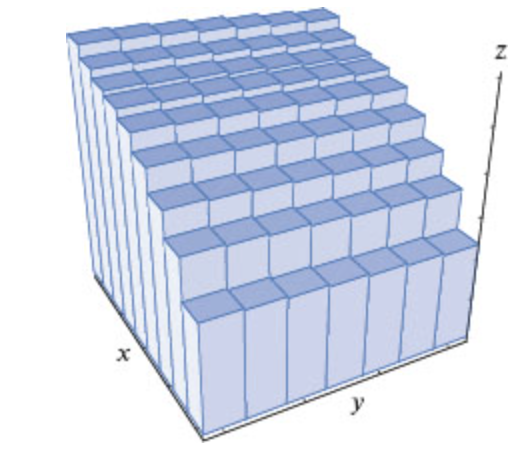
\includegraphics[scale=0.412]{ex16.1.1}
    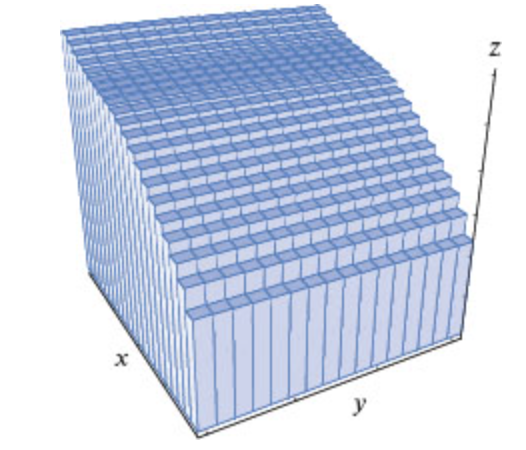
\includegraphics[scale=0.412]{ex16.1.2}
  \end{center}
  Such that if $x, y, z$ represent length and $f$ is positive, then
$$
\begin{aligned}
& \text { Volume under graph } \\
& \text { of } f \text { above region } R
\end{aligned}=\int_R f d A .
$$
}
\ex{Interpretation of the Double Integral as Area}{
In the special case that $f(x, y)=1$ for all points $(x, y)$ in the region $R$, each term in the Riemann sum is of the form $1 \cdot \Delta A=\Delta A$ and the double integral gives the area of the region $R$ :
$$ \operatorname{Area}(R)=\int_R 1 d A=\int_R d A $$
}
\newpage
\ex{Interpretation of the Double Integral as Average Value}{
As in the one-variable case, the definite integral can be used to define the average value of a function:
$$\begin{gathered}\text { Average value of } f \\ \text { on the region } R\end{gathered}=\frac{1}{\text { Area of } R} \int_R f d A$$
\\ We can rewrite this as
$$ \text { Average value } \times \text { Area of } R=\int_R f d A $$
If we interpret the integral as the volume under the graph of $f$, then we can think of the average value of $f$ as the height of the box with the same volume that is on the same base.
\imgg{ex16.3}{0.635}
}
\qs{Over/Under Estimates}{
  Values of $f(x, y)$ are in Table 16.5. Let $R$ be the rectangle $1 \leq x \leq 1.2,2 \leq y \leq 2.4$. Find Riemann sums which are reasonable over and underestimates for $\int_R f(x, y) d A$ with $\Delta x=0.1$ and $\Delta y=0.2$.
  \imgg{qs16.1}{0.635}  
}
\sol Inside Notebook
\qs{}{
  Figure 16.8 shows a contour plot of population density, people per square kilometer, in a rectangle of land $3 \mathrm{~km}$ by $2 \mathrm{~km}$. Estimate the population in the region represented by Figure 16.8.
  \imgg{qs16.2}{0.635}
}
\sol \\
We are given people per square kilometer, such that $\int_R f DA$ is the population as $f$ is the population density, $A$ is the area and $\frac{f}{A} \cdot A$ is people.
We let $\Delta x = \Delta y = 1$ such that we have 6 rectangles.
\begin{align*}
  \text{population} &\approx \Delta x \Delta y [650 + 180 + 400 + 500 + 450 + 100] \\
  &=  1 \text{km}^2 (2280 \frac{\text{ppl}}{\text{km}^2}) = 2280 \text{ people}
\end{align*}
\qs{}{
  Decide (without calculation) whether the integrals are positive, negative, or zero. Let $D$ be the region inside the unit circle centered at the origin, let $R$ be the right half of $D$, and let $B$ be the bottom half of $D$.
  \\1. $\int_D 1 d A$
  \\2. $\int_R 5 x d A$
  \\3. $\int_B 5 x d A$
  \\4. $\int_D\left(y^3+y^5\right) d A$
}
\sol \\
1. Positive, as it is the area of the unit circle. \\
2. Positive, as 5, $x$, $dA$ are all positive. \\ 
3. Zero, as $x$ is symmetric. \\
4. Zero, as $y^3$ and $y^5$ is odd.
\qs{}{
Let $R$ denote the rectangle $[2,10] \times[2,6]$ in the $x y$-plane, and suppose that a thin metal plate having density $\rho(x, y)=x+y$ grams per $\mathrm{cm}^2$ occupies this rectangular region (see diagram to the right). Using $\Delta x=\Delta y=2$, estimate the mass of the metal plate.
Estimate the average density of the metal plate
\imgg{qs16.4}{0.635}
}
\sol We can split the rectangle into 8 squares. Such if that $m = \int_R p(x,y) dA$ we can estimate $m \approx \Delta x \Delta y [\sum_N B_N]$.
Such that $m \approx (2)(2)[6+8+10+12+8+10+12+14] = 320$ g. We can define $f_{\text{avg}} = \rho_{\text{avg}} = \frac{1}{A} m \implies \frac{1}{(4)(8)} 320 = 10$
\newpage
\subsection{Iterated Integrals}
\thm{Double integrals as Iterated Integrals}{
If $R$ is the rectangle $a \leq x \leq b, c \leq y \leq d$ and $f$ is a continuous function on $R$, then the integral of $f$ over $R$ exists and is equal to the iterated integral
$$ \int_R f d A=\int_{y=c}^{y=d}\left(\int_{x=a}^{x=b} f(x, y) d x\right) d y $$
The expression $\int_{y=c}^{y=d}\left(\int_{x=a}^{x=b} f(x, y) d x\right) d y$ can be written $\int_c^d \int_a^b f(x, y) d x d y$.
\double
Such that over $R$ we could have added the columns (fixed $x$) first. This leads to an iterated integral where x is constant in the inner integral instead of y, $\int_R f(x, y) d A=\int_a^b\left(\int_c^d f(x, y) d y\right) dx$.
\\\\ It does not matter in which order we integrate over a rectangular region $R$; in other words, we can add up the columns first or rows first.
$$ \int_R f d A=\int_c^d\left(\int_a^b f(x, y) d x\right) d y=\int_a^b\left(\int_c^d f(x, y) d y\right) d x $$
}
\qs{}{
Evaluate the integral \\
A) $$\int_0^3 \int_0^4(4 x+3 y) d x d y$$
B) Switch the order of (A). \\
C)
$$ \int_0^1 \int_0^1 y e^{x y} d x d y $$
}
\sol \\
We define our $R$ as $0 \leq y \leq 3, 0 \leq x \leq 4$ \\
A)
$$ \int_0^3 \int_0^4(4 x+3 y) dx dy = \int_0^3 (32+12y) dy = \boxed{150} $$
B)
$$ \int_0^4 \int_0^3(4 x+3 y) dy dx = \int_0^4 (12x+\frac{27}{2}) dx = \boxed{150} $$
C)
We define our $R$ as $0 \leq x \leq 1, 0 \leq x \leq 1$ \\
$$ \int_0^1 \int_0^1 y e^{x y} d x d y  = \int_0^1 (e^y - 1) dy = \boxed{e-2}$$
\newpage
\subsubsection{Double Integrals over General Regions}
\qs{}{
Evaluate the integral
$$ \int_0^2 \int_0^y y d x d y $$
}
\sol \\
We define our $R$ as $0 \leq x \leq y, 0 \leq y \leq 2$, such that we define $R$ as a triangle.
$$ \int_0^2 \int_0^y y d x d y  = \int_0^2 (y^2) dy = \boxed{\frac{8}{3}}$$
We can switch our limits of integration.
$$ \int_0^2 \int_x^2 y d y d x  = \int_0^2 (2 - \frac{x^2}{2}) dx = \boxed{\frac{8}{3}}$$
\ex{Integrating a triangle horizontally and vertically}{
  The density at the point $(x, y)$ of a triangular metal plate, is $\delta(x, y)$. Express its mass as an iterated integral.\\
  The vertical strip that starts at the point $(x, 0)$ ends at the point $(x, 2-2 x)$, because the top edge of the triangle is the line $y=2-2 x$. See Figure 16.16. On this vertical strip, $y$ goes from o to $2-2 x$. Hence, the inside integral is
  $$ \int_0^{2-2 x} \delta(x, y) d y $$
  Finally, since there is a vertical strip for each $x$ between 0 and 1 , the outside integral goes from $x=0$ to $x=1$. Thus, the iterated integral we want is
  $$ \text { Mass }=\int_0^1 \int_0^{2-2 x} \delta(x, y) d y d x $$
  \imgg{ex16.4.1}{0.635}
  We could have chosen to integrate in the opposite order, keeping $y$ fixed in the inner integral instead of $x$. The limits are formed by looking at horizontal strips instead of vertical ones, and expressing the $x$-values at the end points in terms of $y$. To find the right endpoint of the strip, we use the equation of the top edge of the triangle in the form $x=1-\frac{1}{2} y$. Thus, a horizontal strip goes from $x=0$ to $x=1-\frac{1}{2} y$. Since there is a strip for every $y$ from o to 2 , the iterated integral is
  $$ \text { Mass }=\int_0^2 \int_0^{1-\frac{1}{2} y} \delta(x, y) d x d y $$
  \imgg{ex16.4.2}{0.635}
  }
\nt{
\textbf{Limits on Iterated Integrals} \\
- The limits on the outer integral must be constants. \\
- The limits on the inner integral can involve only the variable in the outer integral. For example, if the inner integral is with respect to $x$, its limits can be functions of $y$. \\
\textbf{Steps on how to get limits of integration} \\
1. Draw the region, $R$ function is being integration over. \\ 
2. If outer limits are $x$ 's, walk left to right and see what $y$ hits. \\
3. If outer limits are $y$ 's, walk bottom to top and see what $x$ hits.
}
\qs{}{
Sketch the region and integrate
$$ \int_0^6 \int_{x / 3}^2 x \sqrt{y^3+1} dy dx $$
}
\sol Our region is $0 \leq x \leq 6, \frac{x}{3} \leq y \leq 2$ \\
$\int_{x / 3}^2 x \sqrt{y^3+1} dy$ is not a trivial integral, such that we can switch the order of integration. Hint: for u-sub.
$$ \int_0^2 \int_{0}^{3y} x \sqrt{y^3+1} dx dy = \int_0^2 (\frac{9}{2} y^2 \sqrt{y^3 +1}) dy = \boxed{26}$$
\qs{}{
Write $\int_R f d A$ as an iterated integral For the shaded region, $R$.
\imgg{qs16.8}{0.45}
}
\sol In notebook.
\qs{}{
Evaluate the integral by reversing the order of integration.
$$ \int_0^8 \int_{\sqrt[3]{y}}^2 \frac{1}{1+x^4} d x d y $$
}
\sol We define $R$ as $0 \leq y \leq 8, \sqrt[3]{y} \leq x \leq 2$. In notebook.
\qs{}{
Evaluate the integral by reversing the order of integration.
$$ \int_0^3 \int_{y^2}^9 y \sin \left(x^2\right) d x d y $$
}
\sol In notebook
\qs{}{
  Integrate $f(x.y) =xy$ over the region $R$.
}
\subsection{Triple Integrals}
\dfn{Triple Integral as an Iterated Integral}{
$$ \int_W f d V=\int_p^q\left(\int_c^d\left(\int_a^b f(x, y, z) d x\right) d y\right) d z $$
where $y$ and $z$ are treated as constants in the innermost $(d x)$ integral, and $z$ is treated as a constant in the middle $(d y)$ integral. Other orders of integration are possible.
}
\ex{Interpretation of Triple Integrals as Infentesimal Boxes times $f$}{
First we subdivide $W$ into smaller regions, then we multiply the volume of each region by a value of the function in that region, and then we add the results. For example, if $W$ is the box $a \leq x \leq b, c \leq y \leq d, p \leq z \leq q$, then we subdivide each side into $n, m$, and $l$ pieces, thereby chopping $W$ into $n m l$ smaller boxes.
\imgg{ex16.5}{0.57}
The volume of each smaller box is
$$ \Delta V=\Delta x \Delta y \Delta z $$
where $\Delta x=(b-a) / n$, and $\Delta y=(d-c) / m$, and $\Delta z=(q-p) / l$. Using this subdivision, we pick a point $\left(u_{i j k}, v_{i j k}, w_{i j k}\right)$ in the $i j k$-th small box and construct a Riemann sum
$$ \sum_{i, j, k} f\left(u_{i j k}, v_{i j k}, w_{i j k}\right) \Delta V$$
If $f$ is continuous, as $\Delta x, \Delta y$, and $\Delta z$ approach o, this Riemann sum approaches the definite integral, $\int_W f d V$, called a triple integral, which is defined
$$ \int_W f d V =\lim _{\Delta x, \Delta y, \Delta z \rightarrow 0} \sum_{i, j, k} f\left(u_{i j k}, v_{i j k}, w_{i j k}\right) \Delta x \Delta y \Delta z $$
For example, mass is density times volume, where we define the density at any point using $f$. Such that $\int_W f dV$ is the mass of the solid/$\RR^3$ region $W$.
}
\nt{
\textbf{Limits on Triple Integrals} \\
- The limits for the outer integral are constants. \\
- The limits for the middle integral can involve only one variable (that in the outer integral). \\
- The limits for the inner integral can involve two variables (those on the two outer integrals). \\
\textbf{Same as the Double Integral}
- If $\rho(x, y, z)$ is density, then $\int_W \rho d V$ is the total quantity in the solid region $W$.\\
- $\int_W 1 d V$ is the volume of the solid region $W$.
}
\qs{}{
  A cube $\mathrm{C}$ has sides of length $4 \mathrm{~cm}$ and is made of a material of variable density. If one corner is at the origin and the adjacent corners are on the positive $x, y$, and $z$ axes, then the density at the point $(x, y, z)$ is $\delta(x, y, z)=1+x y z \mathrm{~g} / \mathrm{cm}^3$. Find the mass $(m)$ of the cube.
}
\sol 
\begin{align*}
m = \int_C \rho dV &= \int_0^4 \int_0^4 \int_0^4 (1+xyz) dx dy dz \\
&= \int_0^4 \int_0^4 (4+8yz) dy dz \\
&= \int_0^4 (16+64z) dz \\
&= \boxed{576 \text{ g}}
\end{align*}
\qs{}{
  Set up an iterated integral to compute the mass of the solid cone bounded by $z=\sqrt{x^2+y^2}$ and $z=3$, if the density is given by $\delta(x, y, z)=z$.
}
\sol In notebook.
\qs{}{
Sketch the region of integration\\
A) $$ \int_{-1}^1 \int_0^1 \int_{-\sqrt{1-z^2}}^{\sqrt{1-z^2}} f(x, y, z) d y d z d x $$
B) $$ \int_0^1 \int_{-\sqrt{1-z^2}}^{\sqrt{1-z^2}} \int_0^{\sqrt{1-x^2-z^2}} f(x, y, z) d y d x d z$$
}
\qs{}{
Write a triple integral, including limits, that gives the specified volume. \\
A) Between $2 x+2 y+z=6$ and $3 x+4 y+z=6$ and above $x+y \leq 1, x \geq 0, y \geq 0$. \\
B) Between the top portion of the sphere $x^2+y^2+z^2=9$ and the plane $z=2$.
}
\qs{}{
  Find the volume of the region bounded by $z=x^2$, $0 \leq x \leq 5$, and the planes $y=0, y=3$, and $z=0$.
}
\subsection{Double Integrals in Polar Coordinates}
\dfn{Double Integrals in Polar Coordinates}{
  A rectangular grid is constructed from vertical and horizontal lines of the form $x=k$ (a constant) and $y=l$ (another constant). In polar coordinates, $r=k$ gives a circle of radius $k$ centered at the origin and $\theta=l$ gives a ray emanating from the origin (at angle $l$ with the $x$-axis). A polar grid is built out of these circles and rays. Suppose we want to integrate $f(r, \theta)$ over the region $R$ below
  \imgg{ex16.6.1}{0.5}
  Choosing $\left(r_{i j}, \theta_{i j}\right)$ in the $\ddot{j}$-th bent rectangle above gives a Riemann sum:
  $$ \sum_{i, j} f\left(r_{i j}, \theta_{i j}\right) \Delta A . $$

If $\Delta r$ and $\Delta \theta$ are small, the shaded region is approximately a rectangle with sides $r \Delta \theta$ and $\Delta r$, so
$$ \Delta A \approx r \Delta \theta \Delta r $$

Thus, the Riemann sum is approximately
$$ \sum_{i, j} f\left(r_{i j}, \theta_{i j}\right) r_{i j} \Delta \theta \Delta r $$

If we take the limit as $\Delta r$ and $\Delta \theta$ approach o, we obtain
$$ \int_R f d A=\int_\alpha^\beta \int_a^b f(r, \theta) r d r d \theta $$
\imgg{ex16.6.2}{0.5}
When computing integrals in polar coordinates, use $x=r \cos \theta, y=r \sin \theta, x^2+y^2=r^2$. Put $d A=r d r d \theta$ or $d A=r d \theta d r$.
}
\newpage
\qs{}{
  Computer the integral of $f(x, y)=1 /\left(x^2+y^2\right)^{3 / 2}$ over the region $R$ shown below
  \imgg{qs16.17}{0.5}
}
\sol
We can define $f(x,y)$ as $f(x,\theta) = \frac{1}{r^3}$.
$$ \int_0^{\frac{\pi}{4}} \int_1^2 \frac{1}{r^3} r dr d\theta = \frac{\pi}{8} $$
\qs{}{
  For each region set up an iterated integral of an arbitrary function $f(x, y)$ over the region, decide which is best to use, polar or rectangular coordinates.
  \imgg{qs16.18}{0.5}
}
\sol \\
A) $$\int_1^3 \int_{-1}^2 f(x,y) dy dx$$
B) $$\int_0^{2\pi} \int_0^3 f(r, \theta) r dr d\theta$$
C) $$ \int_0^2 \int^3_{\frac{1}{2}x -1} f(x,y) dy dx $$
D) $$\int^\pi_{\frac{\pi}{2}} \int_1^2 f(r,\theta) r dr d\theta$$
\qs{}{
Sketch the region of integration shown:\\
A) $$ \int_3^4 \int_{3 \pi / 4}^{3 \pi / 2} f(r, \theta) r d \theta d r $$
B) $$ \int_0^{\pi / 4} \int_0^{1 / \cos \theta} f(r, \theta) r d r d \theta $$
}
\sol In notebook.
\qs{}{
Evaluate the integral, $\int_R\left(x^2-y^2\right) d A$, where $R$ is the first quadrant region between the circles of radius 1 and radius 2 .
}
\sol
\qs{}{
(a) Sketch the region of integration of
$$ \int_0^1 \int_{\sqrt{1-x^2}}^{\sqrt{4-x^2}} x d y d x+\int_1^2 \int_0^{\sqrt{4-x^2}} x d y d x $$
(b) Evaluate the quantity in part (a).
}
\sol In notebook.
\qs{}{
  Find the volume of a solid bounded by the plane $z=0$ and paraboloid $z=1-x^2-y^2$
}
\sol
\newpage
\subsection{Integrals in 3D Shapes}
\subsubsection{Integrals in Cylindrical Coordinates}
\dfn{Relation Between Cartesian and Cylindrical Coordinates}{
Each point in 3-space is represented using $0 \leq r<\infty, 0 \leq \theta \leq 2 \pi,-\infty<z<\infty$.
$$
\begin{aligned}
& x=r \cos \theta, \\
& y=r \sin \theta, \\
& z=z
\end{aligned}
$$
As with polar coordinates in the plane, note that $x^2+y^2=r^2$.
\imgg{dfn16.4}{0.5}
When computing integrals in cylindrical coordinates, put $d V=r d r d \theta d z$. Other orders of integration are also possible.
}
\ex{Fundamental Cylindrical Surfaces Visualized}{
  The surfaces $r=1$ and $r=2$ \\
  The surfaces $\theta = \pi/4$ and $\theta =3\pi/4$ \\
  The surfaces $z=-1$ and $z=3$ \\
  \begin{center}  
  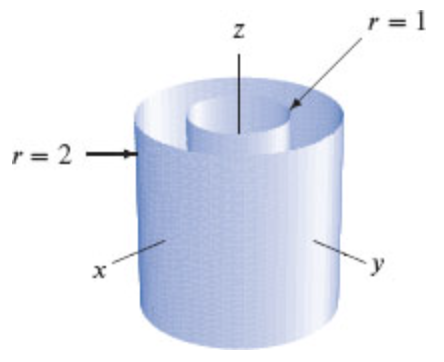
\includegraphics[scale=0.5]{ex16}
  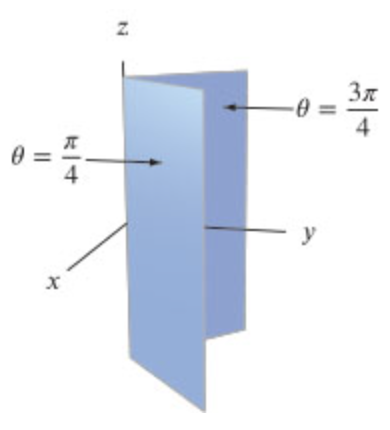
\includegraphics[scale=0.5]{16.6.1}
  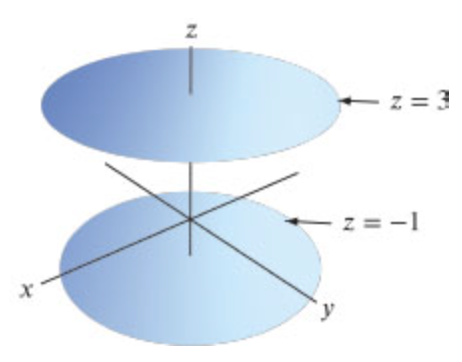
\includegraphics[scale=0.5]{ex16.2}
\end{center}
}
\qs{From Example 16.7}{
  Find the mass of a wedge of cheese cut from a cylinder $4 \mathrm{~cm}$ high and $6 \mathrm{~cm}$ in radius; this wedge subtends an angle of $\pi / 6$ at the center. Its density is $1.2 \mathrm{grams} / \mathrm{cm}^3$.
}
\sol \\
We know that the mass is density times volume. Such that $m = \int_0^4 \int_0^{\pi/2} \int_0^6 1.2 r dr d\theta dz = 45.24$ g
\qs{}{
  Choose a coordinate system and set up a triple integral, including limits of integration, for a density function $f$ over the region given. \\
  A) B) Insert from lecture
}
\sol \\
A) $$\int_0^5 \int_0^3 \int_0^1 f dxdydz $$
B) $$\int_0^1 \int_0^{2\pi} \int_0^4 f r dr d\theta dz $$
\qs{}{
  Evaluate $$\int_{-2}^2 \int_{-\sqrt{4-x^2}}^{\sqrt{4-x^2}} \int_{\sqrt{x^2+y^2}}^2\left(x^2+y^2\right) d z d y d x$$ by analyzing in cylindrical coordinates.
}
\sol In Notebook.
\qs{}{
  Write a triple integral representing the volume above the cone $z=\sqrt{x^2+y^2}$ and below the sphere of radius 2 centered at the origin. Include limits of integration but do not evaluate. Use: Cylindrical coordinates
}
\sol In Notebook.
\qs{}{
  Write a triple integral representing the volume of the region between spheres of radius 1 and 2, both centered at the origin. Include limits of integration but do not evaluate. Use: Cylindrical coordinates. Write answer as difference of two integrals.
}
\sol In Notebook.
\qs{}{
  A sphere has density at each point proportional to the square of the distance of the point from the $z$-axis. The density is $2 \mathrm{gm} / \mathrm{cm}^3$ at a distance of $2 \mathrm{~cm}$ from the axis. What is the mass of the sphere if it is centered at the origin and has radius $3 \mathrm{~cm}$ ?
}
\sol In Notebook.
\subsubsection{Integrals in Spherical Coordinates}
\dfn{Relation Between Cartesian and Spherical Coordinates}{
  Each point in 3 -space is represented using $0 \leq \rho<\infty, 0 \leq \phi \leq \pi$, and $0 \leq \theta \leq 2 \pi$.
$$
\begin{aligned}
& x=\rho \sin \phi \cos \theta \\
& y=\rho \sin \phi \sin \theta \\
& z=\rho \cos \phi \\
& r = \rho \sin \phi
\end{aligned}
$$
Also, $\rho^2=x^2+y^2+z^2$.
\imgg{dfn16.5}{0.5}
}
\thm{}{
  When computing integrals in spherical coordinates, put $d V=\rho^2 \sin \phi d \rho d \phi d \theta$. Other orders of integration are also possible.
}
\myproof We have infentesimal bits, $\Delta \rho$, $\rho \Delta \phi$, and $r \Delta \theta = \rho \sin \phi \Delta \theta$ Such that $dV = \rho^2 \sin \phi d\rho d\phi d\theta$.
\imgg{dfn16.5.1}{0.5}
  
\ex{Fundamental Spherical Surfaces Visualized}{
  The surfaces $\rho=1$ and $\rho=2$ \\
  The surfaces $\theta = \pi/4$ and $\theta =3\pi/4$ \\
  The surfaces $\phi=\pi/6$ and $\phi=2\pi/3$ \\
  \begin{center}  
  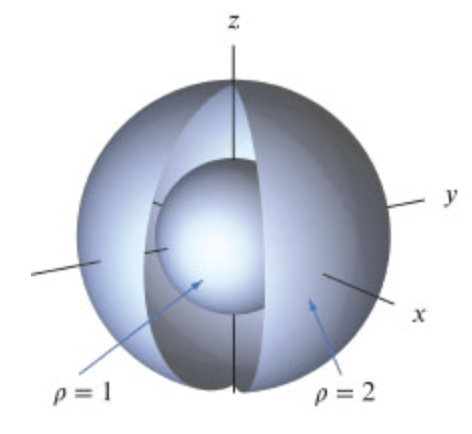
\includegraphics[scale=0.5]{ex16.7.1}
  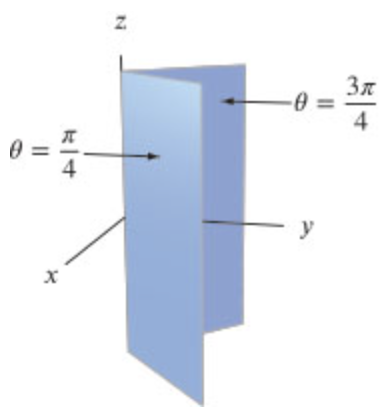
\includegraphics[scale=0.5]{ex16.7.2}
  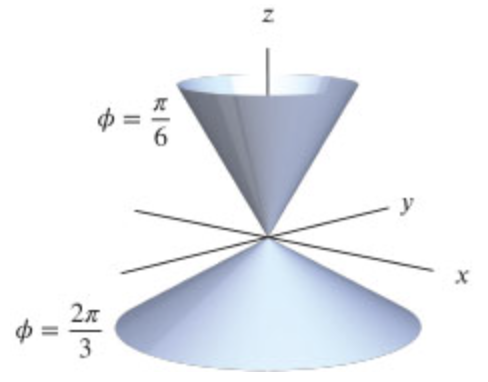
\includegraphics[scale=0.5]{ex16.7.3}
  \end{center}
  Extra: we can say $\rho = 2$ with $ 0 \le \theta \le 3\pi/2$
}
\qs{}{
  Use spherical coordinates to derive the formula for the volume of a sphere of radius $r$.
}
\sol 
$$ V = \int_0^{2\pi} \int_0^\pi \int_0^r \rho^2 \sin \phi dp d\phi d\theta = \frac{4}{3} \pi r^3 $$
\qs{}{
  Choose a coordinate system and set up a triple integral, including limits of integration, for a density function $f$ over the region given.
  \imgg{qs16.30}{0.62}
}
\sol
$$ \int_0^{2\pi} \int_0^{\pi/6} \int_0^3 \rho^2 sin\phi d\rho d\phi d\theta $$
\qs{}{
  Write a triple integral representing the volume of the region between spheres of radius 1 and 2, both centered at the origin. Include limits of integration but do not evaluate. Use spherical coordinates.
}
\sol
$$ \int_0^{2\pi} \int_0^\pi \int_1^2 \rho^2 \sin \phi d \rho d \phi d \theta $$
\qs{}{
  Write a triple integral representing the volume above the cone $z=\sqrt{x^2+y^2}$ and below the sphere of radius 2 centered at the origin. Include limits of integration but do not evaluate. Use spherical coordinates.
}
\sol \\
We have a cone, such that $z = \sqrt{x^2+y^2} = r \implies \rho \cos \phi = \rho \sin \phi \implies \tan \phi = 1 \implies \phi = \frac{\pi}{4} $
$$\int_0^{2\pi} \int_0^{\frac{\pi}{4}} \int_0^2 \rho^2 \sin\phi d\rho d\phi d\theta$$ 
\qs{}{
  Setup the volume of the region shown in each coordinate system
  \imgg{qs16.33}{0.6}
}
\sol \\
FInding where the sphere intersects the cone, we have $ z^2 = x^2 +y^2$ and $z^2 = 1-x^2-y^2$, such that $ x^2 +y^2 = 1-x^2-y^2 \implies r = \sqrt{\frac{1}{2}}$ 
Rectangular:
$$\int_{-\sqrt{\frac{1}{2}}}^{\sqrt{\frac{1}{2}}} \int_{-\sqrt{\frac{1}{2}-x^2}}^{\sqrt{\frac{1}{2}-x^2}} \int_{\sqrt{x^2+y^2}}^{\sqrt{1-x^2-y^2}} dz dy dx $$
Cylindrical:
$$\int_0^{2\pi} \int_0^{\sqrt{\frac{1}{2}}} \int_{r}^{\sqrt{1-r^2}} r dz dr d\theta $$
Spherical:
$$ \int_0^{2\pi} \int_0^{\frac{\pi}{4}} \int_0^1 \rho^2 \sin\phi d\rho d\phi d\theta $$ 
\newpage
\section{Parameters, Coordinates, and Integrals}
\subsection{Parameterized Curves}
Recall "lazy parameterization"; where $y = x^2$, let $x = t$, $y = t^2$. However, $x = \sqrt{t} \implies y = t$, only picks up the right side.
\ex{Parameterized Curves (Circles)}{
  A) $x=\cos t \quad y=\sin t \quad 0 \leq t \leq 2 \pi $ \\
  Visually the parameterization is a circle, traced once, such that it is moving counter clockwise. \\
  To eliminate a parameter we can square both $x$ and $y$, such that $\sin^2(t) + \cos^2(t) = 1 \implies x^2 + y^2 = 1$ \\
  We can takeaway that parameterized curves shoes us direction of motion as $t$ increases.
  \double
  B) $x=\sin 2 t \quad y=\cos 2 t \quad 0 \leq t \leq 2 \pi $ \\
  Subsequently the same, however, we start at (0,1) and goes around twice.
  $$ x=2 \cos t+1 \quad y=2 \sin t+3 \quad 0 \leq t \leq 2 \pi $$
  In the example above, 2 is the radius and $+c$ is the shift.
}
\qs{}{
Give the parameterization of \\
A) a unit circle in the $x y$-plane with center at the origin. \\
B) a circle of radius 5 in the $x z$-plane with center at the origin. \\
C) a circle of radius 3 parallel to the yz-plane with center at $(6,7,8)$. \\
D) a circle of radius 2 parallel to the $x y$-plane with center $(0,0,1)$ traversed counterclockwise when viewed from below.
}
\sol \\
A) Let $x = \cos t$, $y = \sin t$, and $z =0$. \\
B) Let $x = 5 \cos t$, $y = 0$, and $z = 5 \sin t$. \\
C) Let $x = 6$, $y = 3 \cos t + 7$, and $z = 3 \sin t + 8$ \\
D) Let $x = 2\sin t$, $y = 2 \cos t$, and $z = 1$. 
\dfn{Parametric Equations of a Line}{
  Through the point $\left(x_0, y_0, z_0\right)$ and parallel to the vector $\overrightarrow{a i}+\overrightarrow{b j}+\overrightarrow{c k}$ are
  $$ x=x_0+a t, \quad y=y_0+b t, \quad z=z_0+c t $$}
\qs{}{
  A) Find parametric equations for the line in the direction of $3 \vec{\imath}-3 \vec{\jmath}+\vec{k} \text { through }(1,2,3) $ \\
  B) Find parametric equations for the line parallel to the $z \text {-axis through }(1,0,0) $
}
\sol\\
A) We can say the direction vector is the rate of change per $t$. Such that $x = 1+3t$, $y = 2-3t$, and $z = 3+t$. \\
B) $x = 1 + 0t$, $y = 0 + 0t$, and $z = 0 + 1t$.
\qs{}{
  Find parametric equations for the line through the points $(2,3,-1) \text { and }(5,2,0)$
}
\sol We find the vector $\vec{v} = <3,-1,1>$, using the point (2,3,-1), $x = 2+3t$, $y=3-t$, $-1+t$. \\
If all we wanted was the line segment between the points, we could keep $0 \le t \le 1$. \\
If we wanted to reverse the direction we can make the vector negative, $\vec{v} = <-3,1,-1>$.
\dfn{Parametric Equation of a Line in Vector Form}{
  The line through the point with position vector $\overrightarrow{r_0}=x_0 \vec{i}+y_0 \vec{j}+z_0 \vec{k}$ in the direction of the vector $\vec{v}=\overrightarrow{a i}+\overrightarrow{b j}+\overrightarrow{c k}$ has parametric equation
  $$ \vec{r}(t)=\overrightarrow{r_0}+\overrightarrow{t v} $$
}
\ex{Helix Vector Function}{
  In the helix example we have $x = \cos t$, $y = \sin t$, and $z = t$. \\
  Such that, $\vec{r} (t) = (\cos t) \ihat + (\sin t) \jhat + (t) \khat$ \\
  We can say that the output is the position vector of said output point from the origin.
}
\qs{}{
  Are the lines given parallel? Do they intersect? \\
  Line 1: $x=-1+t \quad y=1+2 t \quad z=5-t$ \\
  Line 2: $x=2+2 t \quad y=4+t \quad z=3+t$
}
\sol \\
In line 1: $\vec{r}(t) = <-1,1,5> + t<1,2,-1>$ \\
In line 2: $\vec{r}(t) = <2,4,3> + t<2,1,1>$ \\
We know that for lines to be parallel the direction vectors must be constant multiples of each other, therefore, they are not parallel.
\double
Accounting for different $t$ values, \\
$-1 +t_1 = 2+2t_2$, $1+2t=4t_2$, and $5-t_1=3+t_2$. \\
Solving for one linear equation we get, $t_1 = 1$ and $t_2 = 2$. \\
However, we can see that the lines do not intersect, because the $z$ values are different.
\dfn{Parameterization of Surfaces}{
  In general, we will have
  $$ x=f_1(s, t) \quad y=f_2(s, t) \quad z=f_3(s, t) $$
or write it using position vectors as
$$ \overrightarrow{\mathrm{r}}(s, t)=f_1(s, t) \vec{\imath}+f_2(s, t) \vec{\jmath}+f_3(s, t) \vec{k} $$
}
\qs{}{
  A) Parameterize a cylinder of radius 3 , with central axis the $z$-axis. \\
  B) Parameterize the lower part of the hemisphere $x^2+y^2+z^2=9$.
}
\sol \\
A) We define $x=3\cos t$, $y=3 \sin t$, and $z = s$ (as to not create a spiral). \\
B) The lazy way we can say that $x=s$, $y=t$, and $z=-\sqrt{9-x^2-y^2}$. \\
For spherical coordinates, $x=3 \sin \phi \cos \theta$, $y=3 \sin \phi \sin \theta$, and $z=3 \cos \phi$. Where $\frac{\pi}{2} \le \phi \le \pi$ and $0 \le \theta \le 2\pi$.
\dfn{Parameterizating Planes}{
  The plane through the point with position vector $\vec{r}_0$ and containing the two nonparallel vectors $\vec{v}_1$ and $\vec{v}_2$ has parameterization
  $$ \vec{r}(s, t)=\vec{r}_0+s \vec{v}_1+t \vec{v}_2 $$
}
\qs{}{
  A) Give parametric equations for the plane through the point with position vector $\vec{r}_0$ and containing the vectors $\vec{v}_1$ and $\vec{v}_2$.
  $$ \vec{r}_0=\vec{i}+\vec{j}+\vec{k}, \vec{v}_1=\vec{i}-\vec{k}, \vec{v}_2=-\vec{j}+\vec{k} $$
  B) Parameterize the plane that contains the three points
  $$ (1,2,3),(2,5,8),(5,2,0)$$
}
\sol \\
A) We can say initial is $<1,1,1>$, $\vec{v_1} = <1,0,-1>$ and $\vec{v_2} = <0,-1,1>$. \\
$x = 1 + s$, $y = 1 - t$, and $z = 1 - s + t$. \\
Defining the vector valued function: $\vec{r}(s,t) = (1+s)\ihat + (1-t)\jhat + (1-s+t)\khat$
\double
B) Let $\vec{v_1} = <1,3,5>$ and $\vec{v_2} = <4,0,-3>$. Using (1,2,3) as $\vec{r_0} = <1,2,3>$. \\
$x = 1 + t + 4s$, $y = 2 + 3t$, and $z = 3 + 5t - 3s$. \\
\subsection{Motion, Velocity, Acceleration}
We can define the instantaneous velocity as $\vec{v}(t) = \lim_{\Delta t \to 0} \dfrac{\Delta \vec{r}}{\Delta r} = \dfrac{\vec{r}(t+\Delta t) - \vec{r}(t)}{\Delta t}$. Such that $\nabla (t) = \vec{r}'(t) = \dfrac{d\vec{r}}{dt}$. \\
\dfn{The Velocity \& Acceleration Vector}{
- The magnitude of $\vec{v}$ is the speed of the object. \\
- The direction of $\vec{v}$ is the direction of motion. \\
Thus, the speed of the object is $\|\vec{v}\|$ and the velocity vector is tangent to the object's path.
\imgg{dfn17.5}{0.5}
$$ \vec{v}(t) = \vec{r}'(t) = <f'(t),g'(t),h'(t)> = <\frac{dx}{dt}, \frac{dy}{dt}, \frac{dz}{dt}>$$
$$ \vec{a}(t) = <f''(t),g''(t),h''(t)> = <\frac{d^2x}{dt^2}, \frac{d^2y}{dt^2}, \frac{d^2z}{dt^2}>$$
}
\qs{}{
Find the velocity and acceleration vectors.
$$ x=2+3 t^2, y=4+t^2, z=1-t^2 $$
}
\sol \\
$\vec{r}(t) = <2+3t^2,4+t^2,1-t^2>$, such that $\vec{v} = <6t,2t,-2t>$ and $\vec{a} = <6,2,-2>$.
\qs{}{
Find the velocity vector, the speed, and the times at which the particle stops.
$$ x=3 \sin ^2 t, y=\cos t-1, \quad z=t^2 $$
}
\sol \\
$\vec{v}(t) = <6\sin t \cos t, -\sin t, 2t>$, such that $||\vec{v}|| = \sqrt{36 \sin^2 t \cos^2 t + \sin^2 t + 4t^2}$. \\
We could set each component of the velocity vector to 0 to determine when the particle stops. \\
Where $6\sin t \cos t =0$, $t=n\pi$ and $t=(2n+1)\frac{\pi}{2}$, $n \in \ZZ$. \\
$-\sin t = 0$, $t=pi$ and $2t = 0$, $t=0$. \\
Such that all values are 0 at $t=0$.
\qs{}{
  A particle moves on a circle of radius $5 \mathrm{~cm}$, centered at the origin, in the $x y$-plane ( $x$ and $y$ measured in centimeters). It starts at the point $(0,5)$ and moves counterclockwise, going once around the circle in 8 seconds. \\
  (a) Write a parameterization for the particle's motion. \\
  (b) What is the particle's speed? Give units.
}
\sol \\
Let $x = -5 \sin t$ and $y = \cos t$. Where $y= a\sin bt$, we know that period is $T = \frac{2\pi}{b}$. Such that $8 = \frac{2\pi}{b} \implies b = \frac{\pi}{4}$.
We can say that $x = -5 \sin \frac{\pi}{4} t$ and $y = 5 \cos \frac{\pi}{4} t$. Or $\vec{r}(t) = <-5 \sin \frac{\pi}{4} t, 5 \cos \frac{\pi}{4} t>$. \\
Finding velocity, $\vec{v}(t) = <-5 \frac{\pi}{4} \cos \frac{\pi}{4} t, -5 \frac{\pi}{4} \sin \frac{\pi}{4} t>$. The speed $||\vec{v}|| = \frac{5\pi}{4}$ cm/s counterclockwise. \\
A simpler way, we can say the distance around the circle is $2\pi r = 10\pi$ cm. Such that the speed is $\frac{10\pi}{8} = \frac{5\pi}{4}$ cm/s.
\dfn{Uniform Circular Motion}{
For a particle whose motion is described by $\vec{r}(t)=R \cos (\omega t) \vec{i}+R \sin (\omega t) \vec{j}$ \\
- Motion is in a circle of radius $R$ with period $2 \pi /|\omega|$. \\
- Velocity, $\vec{v}$, is tangent to the circle and speed is constant $\|\vec{v}\|=|\omega| R$. \\
- Acceleration, $\vec{a}(t)$, points toward the center of the circle with $\|\vec{a}\|=\|\vec{v}\|^2 / R$.
}
\dfn{Motion in a Straight Line}{
For a particle whose motion is described by $\vec{r}=\vec{r}_0+t \vec{v}$. \\
- Motion is along a straight line through the point with position vector $\vec{r}_0$ parallel to $\vec{v}$. \\
- Velocity, $\vec{v}$, and acceleration, $\vec{a}$, are parallel to the line.
}
\qs{}{
  A particle starts at the point $P=(3,2,-5)$ and moves along a straight line toward $Q=(5,7,-2)$ at a speed of $5 \mathrm{~cm} / \mathrm{sec}$. Let $x, y, z$ be measured in centimeters. \\
  (a) Find the particle's velocity vector. \\
  (b) Find parametric equations for the particle's motion.
}
\sol \\
$\vec{PQ} = <2,5,3> = \vec{v}(t)$. Such that $\vec{r}_0 + t \vec{v} = <3,2,-5> + t<2,5,3> = <3+2t,2+5t,-5+3t>$ \\
But, the $||v|| = \sqrt{38} \ne 5$. So we have to unitize, $\vec{u} = \vec{v}(t) = <\frac{10}{\sqrt{28}}, \frac{25}{\sqrt{28}}, \frac{15}{\sqrt{28}}>$. \\
Therefore, $\vec{r}(t) = <3,2,-5> + t<\frac{10}{\sqrt{28}}, \frac{25}{\sqrt{28}}, \frac{15}{\sqrt{28}}>$.
\dfn{The Length of a Curve}{
  $$\text{distance} = \int_a^b ||\vec{v}(t)|| dt = C$$
  If the particle doesn't stop and reverse direction than direction = length of the curve.
}
\qs{}{
  Find the length of the curve \\
  A) $x=5 \cos t, y=5 \sin t \quad 0 \leq t \leq 2 \pi$ \\
  B)$x=3+5 t, \quad y=1+4 t, \quad z=3-t \quad 1 \leq t \leq 2$
}
\sol \\
A) $L = \int_0^{2\pi} \sqrt{25\sin^2 t + 25 \cos^2 t} dt = 10\pi$. We could also say $C = 2\pi r = 10\pi$.
\double
B) $\vec{v} = <5,4,-1>$, such that $L = \int_1^2 \sqrt{25+16+1} dt = \sqrt{42}$
\qs{}{
  Suppose $\vec{r}(t)=\cos t \vec{i}+\sin t \vec{j}+2 t \vec{k}$ represents the position of a particle on a helix, where $z$ is the height of the particle above the ground. \\
(a) Is the particle ever moving downward? When? \\
(b) When does the particle reach a point 10 units above the ground? \\
(c) What is the velocity of the particle when it is 10 units above the ground? \\
(d) When it is 10 units above the ground, the particle leaves the helix and moves along the tangent. Find parametric equations for this tangent line.
}
\sol \\
a) If $t>0 \implies 2t>0$, always moving up. I.E. the derivative of the $\khat$ component is $2>0$. \\
b) $2t = 10 \implies t = 5$. \\
c) $\vec{v}(t)= <-\sin t, \cos t, 2>$, such that $\vec{v}(5) = <-\sin 5, \cos 5, 2>$ \\
d) at $t=5$, $\vec{r}(5) = <\cos 5, \sin 5, 10> = \vec{r_0}$, such that $<\cos 5, \sin 5, 10> + (t-5)<-\sin 5, \cos 5, 2>$. \\
$x = \cos 5 - (\sin 5) (t-5)$, $y = \sin 5 + (\cos 5) (t-5)$, and $z = 10 + 2(t-5)$.

\subsection{Vector Fields}
\dfn{Vector Field}{
  A vector field in 2-space is a function $\vec{F}(x, y)$ whose value at a point $(x, y)$ is a 2-dimensional vector. Similarly, a vector field in 3 -space is a function $\vec{F}(x, y, z)$ whose values are 3 -dimensional vectors.
}
\nt{
  Notice the arrow over the function, $\vec{F}$, indicating that its value is a vector, not a scalar. We often represent the point $(x, y)$ or $(x, y, z)$ by its position vector $\vec{r}$ and write the vector field as $\vec{F}(\vec{r})$.
}
\qs{}{
  Sketch the vector field in 2 -space given by $\vec{F}(x, y)=x \vec{j}$
}
\sol In notebook.
\qs{}{
  A) $\vec{F}(x, y)=x \vec{\imath}+y \vec{\jmath}$ \\
  B) How is the vector field $\vec{F}(x, y)=\frac{x \vec{\imath}+y \vec{\jmath}}{\sqrt{x^2+y^2}}$ different from the one above?
}
\sol In notebook.\\
A is often written as $\vec{F}(\vec{r}) = \vec{r}$ and B as $\vec{F}(\vec{r}) = \frac{\vec{r}}{||\vec{r}||}$
\qs{}{
  Sketch the vector field in 2-space given by $F(x, y)=-y \ihat+x \jhat$
}
\sol Sketch in notebook. Looking at $||\vec{F}|| = \sqrt{y^2 +x^2}$; the distance from the origin. Such that drawing a circle on the graph, all the vectors inside that circle are the same length. Therefore as we move away from the origin, the vectors get longer.
The direction of $\vec{F}$ at each point is orthoginal to the position vector. $\vec{F} \cdot \vec{r} = 0$.
\subsection{The Flow of a Vector Field}
\dfn{Flow Line (aka integral curve, streamline)}{
  A flow line of a vector field $\vec{v}=\vec{F}(\vec{r})$ is a path $\vec{r}(t)$ whose velocity vector equals $\vec{v}$. Thus,
  $$ \vec{r}^{\prime}(t)=\vec{v}=\vec{F}(\vec{r}(t))$$
  The flow of a vector field is the family of all of its flow lines.
}
\end{document}